\documentclass[9pt,letter]{article}
\usepackage{lmodern}
\usepackage{amssymb,amsmath}
\usepackage{ifxetex,ifluatex}
\usepackage{fixltx2e} % provides \textsubscript
\ifnum 0\ifxetex 1\fi\ifluatex 1\fi=0 % if pdftex
  \usepackage[T1]{fontenc}
  \usepackage[utf8]{inputenc}
\else % if luatex or xelatex
  \ifxetex
    \usepackage{mathspec}
  \else
    \usepackage{fontspec}
  \fi
  \defaultfontfeatures{Ligatures=TeX,Scale=MatchLowercase}
\fi
% use upquote if available, for straight quotes in verbatim environments
\IfFileExists{upquote.sty}{\usepackage{upquote}}{}
% use microtype if available
\IfFileExists{microtype.sty}{%
\usepackage{microtype}
\UseMicrotypeSet[protrusion]{basicmath} % disable protrusion for tt fonts
}{}
\usepackage[margin=.75in]{geometry}
\usepackage{hyperref}
\hypersetup{unicode=true,
            pdftitle={Assignment 2: Data Visualization},
            pdfborder={0 0 0},
            breaklinks=true}
\urlstyle{same}  % don't use monospace font for urls
\usepackage{color}
\usepackage{fancyvrb}
\newcommand{\VerbBar}{|}
\newcommand{\VERB}{\Verb[commandchars=\\\{\}]}
\DefineVerbatimEnvironment{Highlighting}{Verbatim}{commandchars=\\\{\}}
% Add ',fontsize=\small' for more characters per line
\usepackage{framed}
\definecolor{shadecolor}{RGB}{248,248,248}
\newenvironment{Shaded}{\begin{snugshade}}{\end{snugshade}}
\newcommand{\KeywordTok}[1]{\textcolor[rgb]{0.13,0.29,0.53}{\textbf{#1}}}
\newcommand{\DataTypeTok}[1]{\textcolor[rgb]{0.13,0.29,0.53}{#1}}
\newcommand{\DecValTok}[1]{\textcolor[rgb]{0.00,0.00,0.81}{#1}}
\newcommand{\BaseNTok}[1]{\textcolor[rgb]{0.00,0.00,0.81}{#1}}
\newcommand{\FloatTok}[1]{\textcolor[rgb]{0.00,0.00,0.81}{#1}}
\newcommand{\ConstantTok}[1]{\textcolor[rgb]{0.00,0.00,0.00}{#1}}
\newcommand{\CharTok}[1]{\textcolor[rgb]{0.31,0.60,0.02}{#1}}
\newcommand{\SpecialCharTok}[1]{\textcolor[rgb]{0.00,0.00,0.00}{#1}}
\newcommand{\StringTok}[1]{\textcolor[rgb]{0.31,0.60,0.02}{#1}}
\newcommand{\VerbatimStringTok}[1]{\textcolor[rgb]{0.31,0.60,0.02}{#1}}
\newcommand{\SpecialStringTok}[1]{\textcolor[rgb]{0.31,0.60,0.02}{#1}}
\newcommand{\ImportTok}[1]{#1}
\newcommand{\CommentTok}[1]{\textcolor[rgb]{0.56,0.35,0.01}{\textit{#1}}}
\newcommand{\DocumentationTok}[1]{\textcolor[rgb]{0.56,0.35,0.01}{\textbf{\textit{#1}}}}
\newcommand{\AnnotationTok}[1]{\textcolor[rgb]{0.56,0.35,0.01}{\textbf{\textit{#1}}}}
\newcommand{\CommentVarTok}[1]{\textcolor[rgb]{0.56,0.35,0.01}{\textbf{\textit{#1}}}}
\newcommand{\OtherTok}[1]{\textcolor[rgb]{0.56,0.35,0.01}{#1}}
\newcommand{\FunctionTok}[1]{\textcolor[rgb]{0.00,0.00,0.00}{#1}}
\newcommand{\VariableTok}[1]{\textcolor[rgb]{0.00,0.00,0.00}{#1}}
\newcommand{\ControlFlowTok}[1]{\textcolor[rgb]{0.13,0.29,0.53}{\textbf{#1}}}
\newcommand{\OperatorTok}[1]{\textcolor[rgb]{0.81,0.36,0.00}{\textbf{#1}}}
\newcommand{\BuiltInTok}[1]{#1}
\newcommand{\ExtensionTok}[1]{#1}
\newcommand{\PreprocessorTok}[1]{\textcolor[rgb]{0.56,0.35,0.01}{\textit{#1}}}
\newcommand{\AttributeTok}[1]{\textcolor[rgb]{0.77,0.63,0.00}{#1}}
\newcommand{\RegionMarkerTok}[1]{#1}
\newcommand{\InformationTok}[1]{\textcolor[rgb]{0.56,0.35,0.01}{\textbf{\textit{#1}}}}
\newcommand{\WarningTok}[1]{\textcolor[rgb]{0.56,0.35,0.01}{\textbf{\textit{#1}}}}
\newcommand{\AlertTok}[1]{\textcolor[rgb]{0.94,0.16,0.16}{#1}}
\newcommand{\ErrorTok}[1]{\textcolor[rgb]{0.64,0.00,0.00}{\textbf{#1}}}
\newcommand{\NormalTok}[1]{#1}
\usepackage{longtable,booktabs}
\usepackage{graphicx,grffile}
\makeatletter
\def\maxwidth{\ifdim\Gin@nat@width>\linewidth\linewidth\else\Gin@nat@width\fi}
\def\maxheight{\ifdim\Gin@nat@height>\textheight\textheight\else\Gin@nat@height\fi}
\makeatother
% Scale images if necessary, so that they will not overflow the page
% margins by default, and it is still possible to overwrite the defaults
% using explicit options in \includegraphics[width, height, ...]{}
\setkeys{Gin}{width=\maxwidth,height=\maxheight,keepaspectratio}
\IfFileExists{parskip.sty}{%
\usepackage{parskip}
}{% else
\setlength{\parindent}{0pt}
\setlength{\parskip}{6pt plus 2pt minus 1pt}
}
\setlength{\emergencystretch}{3em}  % prevent overfull lines
\providecommand{\tightlist}{%
  \setlength{\itemsep}{0pt}\setlength{\parskip}{0pt}}
\setcounter{secnumdepth}{0}
% Redefines (sub)paragraphs to behave more like sections
\ifx\paragraph\undefined\else
\let\oldparagraph\paragraph
\renewcommand{\paragraph}[1]{\oldparagraph{#1}\mbox{}}
\fi
\ifx\subparagraph\undefined\else
\let\oldsubparagraph\subparagraph
\renewcommand{\subparagraph}[1]{\oldsubparagraph{#1}\mbox{}}
\fi

%%% Use protect on footnotes to avoid problems with footnotes in titles
\let\rmarkdownfootnote\footnote%
\def\footnote{\protect\rmarkdownfootnote}

%%% Change title format to be more compact
\usepackage{titling}

% Create subtitle command for use in maketitle
\newcommand{\subtitle}[1]{
  \posttitle{
    \begin{center}\large#1\end{center}
    }
}

\setlength{\droptitle}{-2em}
  \title{Assignment 2: Data Visualization}
  \pretitle{\vspace{\droptitle}\centering\huge}
  \posttitle{\par}
\subtitle{Azoacha Forcheh, 20558994}
  \author{}
  \preauthor{}\postauthor{}
  \date{}
  \predate{}\postdate{}

\usepackage{booktabs}
\usepackage{longtable}
\usepackage{array}
\usepackage{multirow}
\usepackage[table]{xcolor}
\usepackage{wrapfig}
\usepackage{float}
\usepackage{colortbl}
\usepackage{pdflscape}
\usepackage{tabu}
\usepackage{threeparttable}
\usepackage{graphicx}
\usepackage{color}
\usepackage{booktabs}
\usepackage{longtable}
\usepackage{array}
\usepackage{multirow}
\usepackage[table]{xcolor}
\usepackage{wrapfig}
\usepackage{float}
\usepackage{colortbl}
\usepackage{pdflscape}
\usepackage{tabu}
\usepackage{threeparttable}

\begin{document}
\maketitle

\begin{enumerate}
\def\labelenumi{\arabic{enumi}.}
\tightlist
\item
  Visual fractions can be used to provide a sense of the size of that
  fraction (provided it is not too small). In the document
  \texttt{VisualFractions.pdf}, you will find an introduction to some
  graphical primitives that will allow you to draw some visual fractions
  using circles (the \texttt{VisualFractions.Rmd} contains the code in
  an Rmarkdown file which you might find helpful).
\end{enumerate}

\begin{enumerate}
\def\labelenumi{(\alph{enumi})}
\item
  (10 marks) Read that document and complete the definition of the
  function \(\mathtt{visualFraction(\cdots)}\).

\begin{Shaded}
\begin{Highlighting}[]
\NormalTok{visualFraction <-}\StringTok{ }\ControlFlowTok{function}\NormalTok{(num, }\CommentTok{# the numerator}
\NormalTok{                           den, }\CommentTok{# the denominator}
                           \DataTypeTok{numCol=}\StringTok{"red"}\NormalTok{,}
                           \CommentTok{# numerator colour}
                           \DataTypeTok{denCol=}\StringTok{"white"}\NormalTok{,}
                           \CommentTok{# denominator colour}
                           \DataTypeTok{random=}\OtherTok{FALSE}\NormalTok{,}
                           \CommentTok{# a logical indicating}
                           \CommentTok{# whether the numerator values}
                           \CommentTok{# are to appear at random}
                           \CommentTok{# locations (if TRUE) or not.}
                           \DataTypeTok{ncols =} \OtherTok{NULL}
                           \CommentTok{# number of columns to be}
                           \CommentTok{# used in the array}
\NormalTok{) \{}
  \CommentTok{# begin with some error checking}
  \CommentTok{#}
  \CommentTok{#  Check the logical}
  \ControlFlowTok{if}\NormalTok{ (}\OperatorTok{!}\KeywordTok{is.logical}\NormalTok{(random))}
    \KeywordTok{stop}\NormalTok{(}\KeywordTok{paste}\NormalTok{(}\StringTok{"random must be TRUE or FALSE, not:"}\NormalTok{,}
\NormalTok{               random))}
  \CommentTok{#}
  \CommentTok{#  Check the numerator}
  \ControlFlowTok{if}\NormalTok{ (}\OperatorTok{!}\KeywordTok{is.numeric}\NormalTok{(num))}
    \KeywordTok{stop}\NormalTok{(}\KeywordTok{paste}\NormalTok{(}\StringTok{"num must be a number, not"}\NormalTok{, num))}
  \ControlFlowTok{if}\NormalTok{ (}\KeywordTok{length}\NormalTok{(num) }\OperatorTok{!=}\StringTok{ }\DecValTok{1}\NormalTok{)}
    \KeywordTok{stop}\NormalTok{(}\KeywordTok{paste}\NormalTok{(}\StringTok{"num must be a single number, not of length"}\NormalTok{,}
               \KeywordTok{length}\NormalTok{(num)))}
  \ControlFlowTok{if}\NormalTok{ (}\KeywordTok{floor}\NormalTok{(num) }\OperatorTok{!=}\StringTok{ }\NormalTok{num }\OperatorTok{|}\StringTok{ }\NormalTok{num }\OperatorTok{<}\StringTok{ }\DecValTok{0}\NormalTok{ )}
    \KeywordTok{stop}\NormalTok{(}\KeywordTok{paste}\NormalTok{(}\StringTok{"num must be a non-negative integer, not"}\NormalTok{,}
\NormalTok{               num))}
  \CommentTok{#}
  \CommentTok{#  Check the denominator}
  \ControlFlowTok{if}\NormalTok{ (}\OperatorTok{!}\KeywordTok{is.numeric}\NormalTok{(den))}
    \KeywordTok{stop}\NormalTok{(}\KeywordTok{paste}\NormalTok{(}\StringTok{"den must be a number, not"}\NormalTok{, den))}
  \ControlFlowTok{if}\NormalTok{ (}\KeywordTok{length}\NormalTok{(den) }\OperatorTok{!=}\StringTok{ }\DecValTok{1}\NormalTok{)}
    \KeywordTok{stop}\NormalTok{(}\KeywordTok{paste}\NormalTok{(}\StringTok{"den must be a single number, not of length"}\NormalTok{,}
               \KeywordTok{length}\NormalTok{(den)))}
  \ControlFlowTok{if}\NormalTok{ (}\KeywordTok{floor}\NormalTok{(den) }\OperatorTok{!=}\StringTok{ }\NormalTok{den }\OperatorTok{|}\StringTok{ }\NormalTok{den }\OperatorTok{<}\StringTok{ }\DecValTok{0}\NormalTok{ )}
    \KeywordTok{stop}\NormalTok{(}\KeywordTok{paste}\NormalTok{(}\StringTok{"den must be a non-negative integer, not"}\NormalTok{,}
\NormalTok{               den))}
  \CommentTok{#}
  \CommentTok{#  Check both}
  \ControlFlowTok{if}\NormalTok{ (num }\OperatorTok{>}\StringTok{ }\NormalTok{den)}
    \KeywordTok{stop}\NormalTok{(}\KeywordTok{paste}\NormalTok{(}\StringTok{"num ="}\NormalTok{, num, }\StringTok{"> den ="}\NormalTok{, den))}
  \CommentTok{#}
  \CommentTok{#  Check ncols}
  \CommentTok{#}
  \CommentTok{#  Default is NULL, so if user doesn't supply one let's}
  \CommentTok{#  try to make it close to square (default more cols than rows)}
  \ControlFlowTok{if}\NormalTok{ (}\KeywordTok{is.null}\NormalTok{(ncols)) ncols <-}\StringTok{ }\KeywordTok{ceiling}\NormalTok{(}\KeywordTok{sqrt}\NormalTok{(den))}

  \CommentTok{#  Now check any user supplied value for ncols}
  \ControlFlowTok{if}\NormalTok{ (}\OperatorTok{!}\KeywordTok{is.numeric}\NormalTok{(ncols))}
    \KeywordTok{stop}\NormalTok{(}\KeywordTok{paste}\NormalTok{(}\StringTok{"ncols must be a number, not"}\NormalTok{, ncols))}
  \ControlFlowTok{if}\NormalTok{ (}\KeywordTok{length}\NormalTok{(ncols) }\OperatorTok{!=}\StringTok{ }\DecValTok{1}\NormalTok{)}
    \KeywordTok{stop}\NormalTok{(}\KeywordTok{paste}\NormalTok{(}\StringTok{"ncols must be a single number, not of length"}\NormalTok{,}
               \KeywordTok{length}\NormalTok{(ncols)))}
  \ControlFlowTok{if}\NormalTok{ (}\KeywordTok{floor}\NormalTok{(ncols) }\OperatorTok{!=}\StringTok{ }\NormalTok{ncols }\OperatorTok{|}\StringTok{ }\NormalTok{ncols }\OperatorTok{<}\StringTok{ }\DecValTok{0}\NormalTok{ )}
    \KeywordTok{stop}\NormalTok{(}\KeywordTok{paste}\NormalTok{(}\StringTok{"ncols must be a non-negative integer, not"}\NormalTok{,}
\NormalTok{               ncols))}
  \ControlFlowTok{if}\NormalTok{ (ncols }\OperatorTok{>}\StringTok{ }\NormalTok{den )}
    \KeywordTok{stop}\NormalTok{(}\KeywordTok{paste}\NormalTok{(}\StringTok{"ncols ="}\NormalTok{, ncols,}\StringTok{"> den ="}\NormalTok{, den))}

\NormalTok{  ## If we have ncols columns, we will need}
\NormalTok{  ## nrows rows where}
\NormalTok{  nrows <-}\StringTok{ }\KeywordTok{ceiling}\NormalTok{(den}\OperatorTok{/}\NormalTok{ncols)}

\NormalTok{  ## We'll also need a radius}
\NormalTok{  ## This is size provides spacing for most}
\NormalTok{  radius <-}\StringTok{ }\DecValTok{1}\OperatorTok{/}\NormalTok{(}\DecValTok{2}\OperatorTok{*}\NormalTok{(}\KeywordTok{max}\NormalTok{(nrows,ncols)}\OperatorTok{+}\DecValTok{5}\NormalTok{))}

\NormalTok{  ##}
\NormalTok{  ## Now it's your turn}
\NormalTok{  ## The display should be an nrows x ncols array of den circles}
\NormalTok{  ## }
\NormalTok{  ## If random=FALSE, the first num circles (from the top left of the}
\NormalTok{  ## array and proceeding left to right, then top to bottom) }
\NormalTok{  ## should be coloured numCol, the remainder coloured denCol.}
\NormalTok{  ## }
\NormalTok{  ## If random=TRUE, num circles selected at random in the array}
\NormalTok{  ## should be coloured numCol, the remainder denCol.}
\NormalTok{  ## }
\NormalTok{  ## That is, if we index the array 1 to den from top left by row to bottom}
\NormalTok{  ## right, the indices we would need to colour numCol would be}
  \ControlFlowTok{if}\NormalTok{ (random) \{indices <-}\StringTok{ }\KeywordTok{sample}\NormalTok{(}\DecValTok{1}\OperatorTok{:}\NormalTok{den, num)\} }\ControlFlowTok{else}\NormalTok{ \{indices <-}\StringTok{ }\DecValTok{1}\OperatorTok{:}\NormalTok{num\}}
\NormalTok{  ##}
\NormalTok{  ## INSERT YOUR CODE BELOW:}

\NormalTok{  ## calculating the coordinates of the centers of the circles}
\NormalTok{  centers =}\StringTok{ }\KeywordTok{xy2grid}\NormalTok{(}\DecValTok{1}\OperatorTok{:}\NormalTok{ncols, nrows}\OperatorTok{:}\DecValTok{1}\NormalTok{)}
  \CommentTok{# dividing to make get points within the unit square}
\NormalTok{  centers[,}\DecValTok{1}\NormalTok{] =}\StringTok{ }\NormalTok{centers[,}\DecValTok{1}\NormalTok{]}\OperatorTok{/}\NormalTok{(ncols}\OperatorTok{+}\DecValTok{1}\NormalTok{)}
\NormalTok{  centers[,}\DecValTok{2}\NormalTok{] =}\StringTok{ }\NormalTok{(}\DecValTok{2}\OperatorTok{*}\NormalTok{centers[,}\DecValTok{2}\NormalTok{] }\OperatorTok{-}\StringTok{ }\DecValTok{1}\NormalTok{)}\OperatorTok{/}\NormalTok{(}\DecValTok{2}\OperatorTok{*}\NormalTok{nrows)}

\NormalTok{  ## generating the display}
  \KeywordTok{grid.newpage}\NormalTok{()}
  \ControlFlowTok{for}\NormalTok{ (i }\ControlFlowTok{in} \DecValTok{1}\OperatorTok{:}\NormalTok{den) \{}
    \ControlFlowTok{if}\NormalTok{(i }\OperatorTok\StringTok{ }\NormalTok{indices) \{col =}\StringTok{ }\NormalTok{numCol\} }\ControlFlowTok{else}\NormalTok{ \{col =}\StringTok{ }\NormalTok{denCol\}}
\NormalTok{    xcoord =}\StringTok{ }\NormalTok{centers[i,}\DecValTok{1}\NormalTok{]}
\NormalTok{    ycoord =}\StringTok{ }\NormalTok{centers[i,}\DecValTok{2}\NormalTok{]}
    \KeywordTok{grid.circle}\NormalTok{(}\DataTypeTok{x=}\NormalTok{xcoord,}
                \DataTypeTok{y=}\NormalTok{ycoord,}
                \DataTypeTok{r=}\NormalTok{radius, }
                \DataTypeTok{gp=}\KeywordTok{gpar}\NormalTok{(}\DataTypeTok{fill=}\NormalTok{col))}
\NormalTok{  \}}
\NormalTok{\}}
\end{Highlighting}
\end{Shaded}
\item
  Show the results of your program on \(\frac{3}{100}\) and also on
  \(\frac{37}{1000}\). In each case, show the results
  \textbf{both when } \(\mathtt{random=FALSE}\) \textbf{and when}
  \(\mathtt{random=TRUE}\).

\begin{Shaded}
\begin{Highlighting}[]
\CommentTok{# results for 3/100}
\KeywordTok{visualFraction}\NormalTok{(}\DecValTok{3}\NormalTok{,}\DecValTok{100}\NormalTok{)}
\end{Highlighting}
\end{Shaded}

  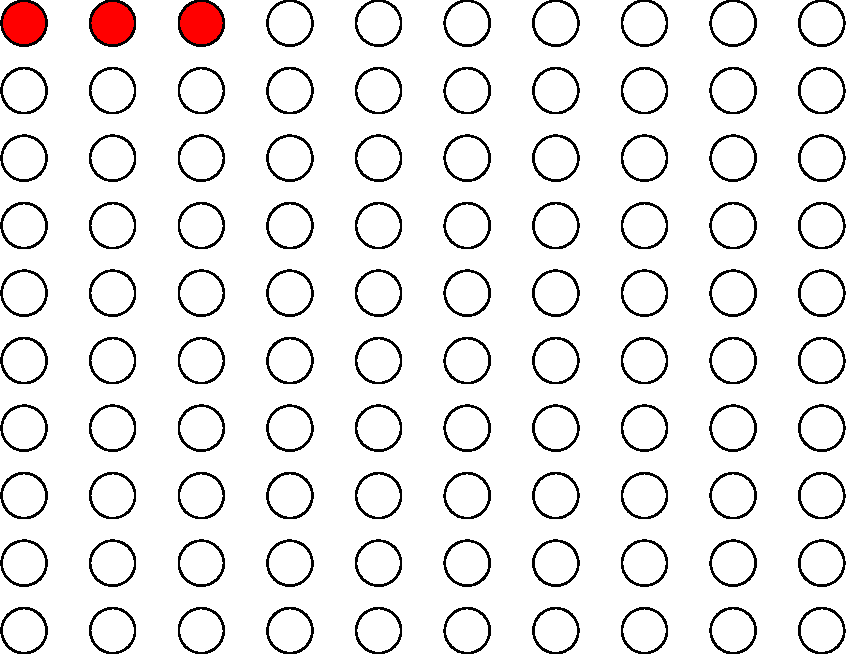
\includegraphics{a2_solutions_files/figure-latex/unnamed-chunk-3-1.pdf}

\begin{Shaded}
\begin{Highlighting}[]
\KeywordTok{visualFraction}\NormalTok{(}\DecValTok{3}\NormalTok{,}\DecValTok{100}\NormalTok{, }\DataTypeTok{random=}\OtherTok{TRUE}\NormalTok{)}
\end{Highlighting}
\end{Shaded}

  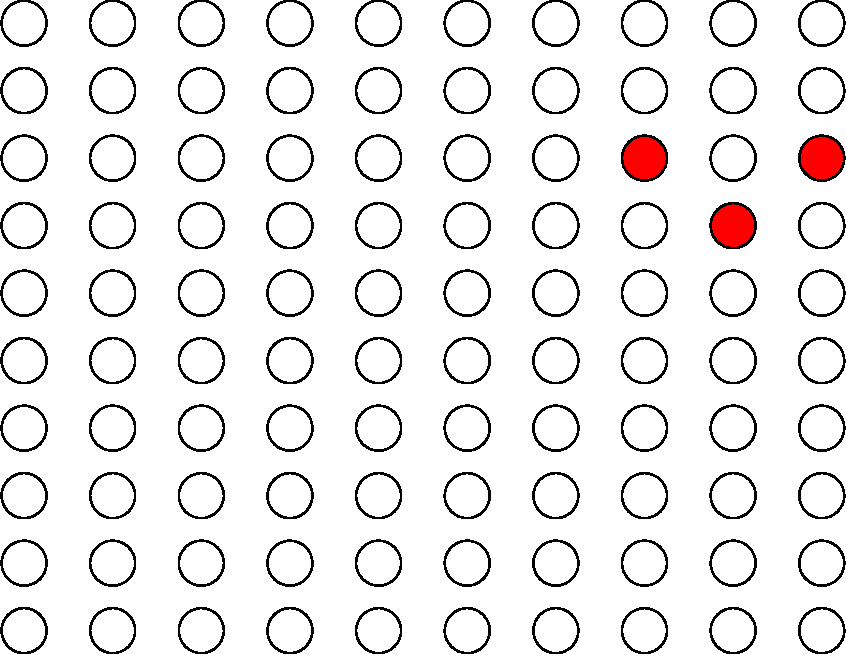
\includegraphics{a2_solutions_files/figure-latex/unnamed-chunk-3-2.pdf}

\begin{Shaded}
\begin{Highlighting}[]
\CommentTok{# results for 37/1000}
\KeywordTok{visualFraction}\NormalTok{(}\DecValTok{37}\NormalTok{,}\DecValTok{1000}\NormalTok{)}
\end{Highlighting}
\end{Shaded}

  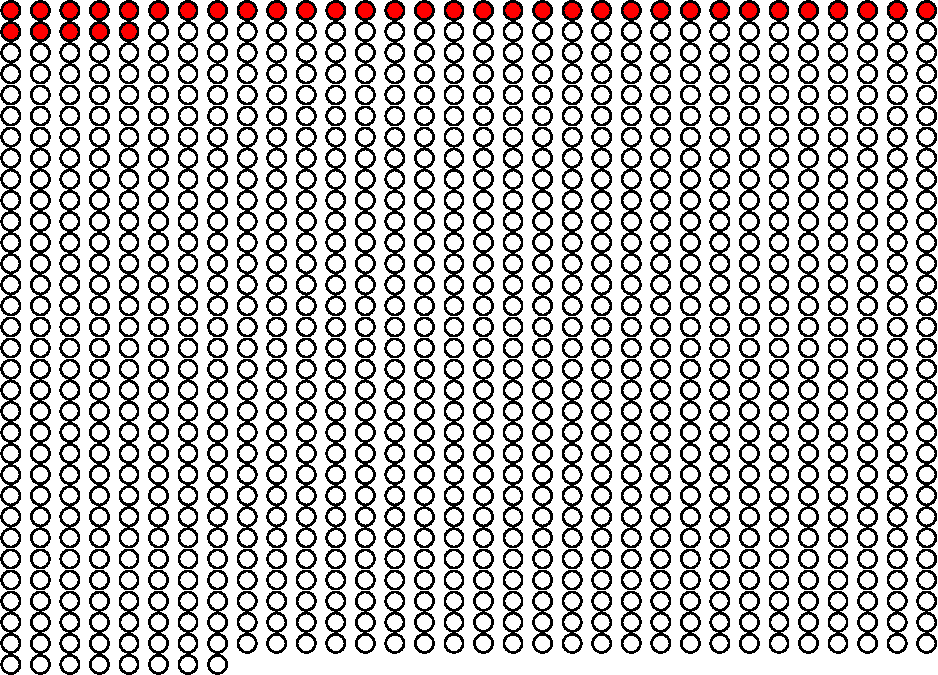
\includegraphics{a2_solutions_files/figure-latex/unnamed-chunk-4-1.pdf}

\begin{Shaded}
\begin{Highlighting}[]
\KeywordTok{visualFraction}\NormalTok{(}\DecValTok{37}\NormalTok{,}\DecValTok{1000}\NormalTok{, }\DataTypeTok{random=}\OtherTok{TRUE}\NormalTok{)}
\end{Highlighting}
\end{Shaded}

  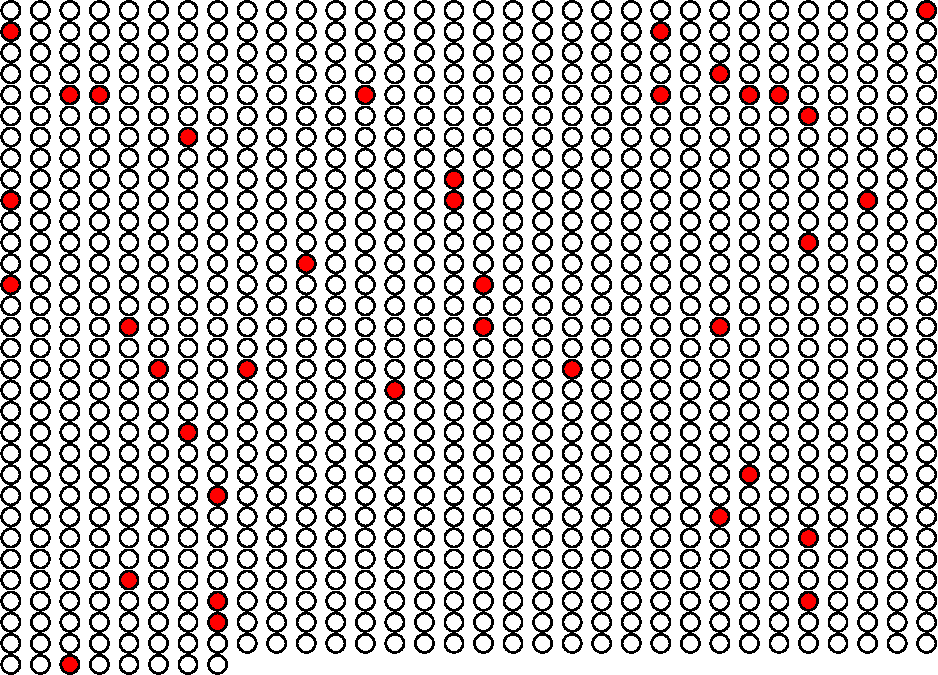
\includegraphics{a2_solutions_files/figure-latex/unnamed-chunk-4-2.pdf}
\item
  (2 marks) Explain why the case \(\mathtt{random=TRUE}\) might be of
  interest.

  For larger denominators, having the overplotted circles be randomly
  spread out makes it easier to quickly visually evaluate/approximate
  what ratio the original fraction was than having them all grouped out
  at the top of the diagram.
\end{enumerate}

\begin{enumerate}
\def\labelenumi{\arabic{enumi}.}
\setcounter{enumi}{1}
\item
  In class, a time scale was used to indicate the average time it would
  take to first win Lotto 649, purchasing 1 ticket per weekly draw.
  Assume that a winning ticket is one which matches the 6 numbers drawn
  from 1 to 49.

  \begin{enumerate}
  \def\labelenumii{(\alph{enumii})}
  \tightlist
  \item
    (1 mark) Suppose \(p\) is the probability of winning the grand
    prize. Write down the value for \(p\) for Lotto 649. The numbers are
    being drawn without replacement and their order does not matter, so
    the number of possible combinations is: \[
    \begin{array}{rcl}
    \binom{49}{6} & = & \frac{49!}{6!(49-6)!}\\
    \\
    & = &  \frac{49!}{6!43!}\\
    \\
    & = & 13,983,816
    \\
    \end{array}
    \]
  \end{enumerate}

  \(\therefore p = \frac{1}{13,983,816}\)

  \begin{enumerate}
  \def\labelenumii{(\alph{enumii})}
  \setcounter{enumii}{1}
  \tightlist
  \item
    (1 mark) Write down the probability of winning
    (\textbf{for the first time}) on the \(n\)th draw (i.e.~losing on
    the first \(n-1\) draws). Let \(X\) be a random variable that
    represents the number of draws up to and including the draw in which
    the player wins for the first time. Then:
  \end{enumerate}

  \[
  X \sim Geo(p) \quad \quad where\ \ p = \frac{1}{13,983,816}
  \] Therefore, the probability of winning (\textbf{for the first time})
  on the \(n\)th draw is:

  \[
  \begin{array}{rcl}
  P(X=n) &=& p(1-p)^{n-1}\\
  \\
  &=& \frac{13,983,815^{n-1}}{13,983,816^{n}}\\
  \\
  &=& \frac{1}{13,983,815} \cdot (\frac{13,983,815}{13,983,816})^{n}
  \end{array}
  \]

  \begin{enumerate}
  \def\labelenumii{(\alph{enumii})}
  \setcounter{enumii}{2}
  \tightlist
  \item
    (1 mark) Determine the expected number of draws you must play (1
    ticket each draw) before winning for the first time. As in (b), let
    \(X\) be a random variable that represents the number of draws up to
    and including the draw in which you wins for the first time. Then,
    the expected number of draws you must play (1 ticket each draw)
    before winning for the first time is \(E(X)\). Since \(X\) follows a
    geometric distribution with probablity \(p\),
  \end{enumerate}

  \[
  \begin{array}{rcl}
  E(X) & = & \frac{1}{p}\\
  \\
  & = & 13,983,816
  \end{array}
  \] \(\therefore\) \textbf{$13,983,816$} is the expected number of
  draws you must play before winning for the first time.

  \begin{enumerate}
  \def\labelenumii{(\alph{enumii})}
  \setcounter{enumii}{3}
  \tightlist
  \item
    (1 mark) Show how the average time to win Lotto 649 when playing 1
    ticket per weekly 649 draw turns into the long wait given for the
    Homo sapiens example (as described in the slides).
  \end{enumerate}
\item
  Colour blindness:

  \begin{enumerate}
  \def\labelenumii{\alph{enumii}.}
  \item
    (3 marks) How well do each of these palettes work for those unable
    to see colour at all? Why?

    The image below shows the monochromatic view of the original
    palettes (generated by the given website).

    \begin{figure}[h]
      \centering
        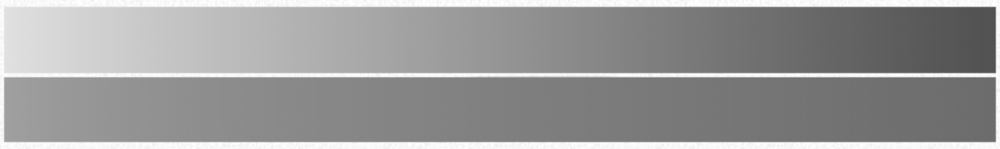
\includegraphics{./img/no_colour}
        \caption{Monochromatic View of Palettes}
    \end{figure}

    Though both are grey palettes with no varying hue, the
    \textbf{yellow to blue} palette works better for those unable to see
    color.

    This is because this palette has opposing, distinguishable
    \textbf{saturation}, which increases from the start to the end of
    the palette. Hence, those unable to see color can use saturation
    instead of hue to distinguish between categories.

    The second palette (the green to red one) however, has very little,
    almost-unnoticeable variation in the saturation of the grey, so
    there is no way that anyone with monochromatic vision will be able
    to tell apart various categories.
  \item
    (3 marks) Which oppositional colour pair seems best over all --
    yellow-blue or green-red? Explain your answer.

    Overall, to benefit the most amount of people, it would be best to
    use the \textbf{green-red} palette.

    \begin{itemize}
    \item No color blindness: both are good as the opposing hues are distinguishable.
    \item Protanopia: 2nd palette is worse (becomes a dark yellow palette with very little saturation variety); first is still a yellow blue palette with distinguishable hues
    \item Deuteranopia: Same result as with protanopia, but 2nd palette is a dark orange palette and 1st is now an orange blue palette
    \item Tritanopia: Both palettes have opposing colors on their opposite ends, but 2nd is better as there is a higher range of constrasting hue along the palette because the red opposes the blue more than the lavender does.
    \end{itemize}

    While the green-red palette is the worse option of the two palettes
    for people with monochromatic vision, it is an extremely rare
    condition - it occurs 1 in 33000 people according to
    colourblindawareness.org. Hence, unless a substantial subset of the
    target viewers of the graphics have monochromatic vision, it is
    overall better to use the \textbf{green-red} palette.
  \item
    (4 marks) Given what we discussed in class about the photo-receptors
    in the human retina, what characteristic of the photo-receptors
    might explain your choice in part (b)? The medium and long cones are
    both able to absorb green and red light to different degrees,
    whereas the short cones are able to absorb purple, blue and green
    light. Hence, most of the cones in the human eye can absorb green
    and red color, and the colors in between those wavelengths, so
    humans would be better able to perceive the colors in the green-red
    palette.
  \end{enumerate}
\item
  Visual representations.

  \begin{enumerate}
  \def\labelenumii{(\alph{enumii})}
  \tightlist
  \item
    The following diagram was produced by the World Health Organization
    few years back.
  \end{enumerate}

  \begin{enumerate}
  \def\labelenumii{\roman{enumii}.}
  \tightlist
  \item
    (4 marks) Suppose the percentages were not actually displayed. What
    visual features of the display are available to the reader to decode
    the numbers presented? Which of these correspond to the percentages?
    \newline
     \newline
     The \textbf{size} of the drops and their \textbf{colors/designs}
    can be used by the reader to decode the presented numbers. \newline
     The color of the drops tells the reader what category of water
    (satisfactory or unsatisfactory) that the percentages would be
    representing. Water is typically depicted as being a vibrant blue,
    so readers would likely be able to use these differences in
    saturation and design to distinguish between the categories that
    each drop represented. The more-saturated blue drop would be decoded
    as satisfactory water, and the less-saturated, pink-dotted drop
    would be decoded as unsatisfactory water. \newline
     As can be seen in the original diagram, the size of the drop
    positively correlates with the percentage displayed. A reader can
    infer that a bigger drop indicates a higher percentage, especially
    since the scale is the same for both years and for both categories
    displayed. \vspace{5mm}
  \item
    (4 marks) From Cleveland and McGill's ordering of elementary tasks
    identify which of these tasks are used where in this diagram. Which
    of these elementary tasks are most likely to be used in decoding the
    numbers by the reader? Comment on the likely accuracy of this
    decoding. \vspace{5mm}

    \begin{itemize}
    \item \textbf{Position on identical but nonaligned scales}: this is used to judge the size of the drops, and hence the magnitude of the numbers/percentages. It is somewhat accuragte for this decoding, as the relative positioning of the drop tells the user how large the magnitude of the numbers are (the higher positioned the drop is, the larger its corresponding percentage's magnitiude.) However, this is only clear when used with the elementary task of judging area.
    \item \textbf{Area}: this is used with the size of drops. It is the most accurate decoding for the magnitude of the numbers, as it is easy to quickly percieve the difference in the area of the drops, and thus decode what percentage the drop may represent.
    \item \textbf{Color hue}: this is used in the design of the drops. It is the most accurate decoding for the category/type of water source being described, as it is the colors being used - blue vs brown and blue with pink dots - have respectively positive and negative connotation to them. Hence, it is easy for readers to quickly decode what category the drops and their numbers correspond to.   
    \end{itemize}

    \vspace{5mm}
  \item
    (4 marks) Create a table representing the same numerical
    information. Give the pros and cons of the table compared to the
    original diagram. (See \texttt{Tables.Rmd} in the folder for this
    assignment)
  \end{enumerate}

\begin{Shaded}
\begin{Highlighting}[]
\KeywordTok{library}\NormalTok{(kableExtra)}
\NormalTok{cleanWater =}\StringTok{ }\KeywordTok{c}\NormalTok{(}\DecValTok{82}\NormalTok{, }\DecValTok{66}\NormalTok{)}
\NormalTok{waterData =}\StringTok{ }\KeywordTok{data.frame}\NormalTok{(}\KeywordTok{c}\NormalTok{(}\StringTok{'Satisfactory'}\NormalTok{, }\StringTok{'Unsatisfactory'}\NormalTok{), }\KeywordTok{rbind}\NormalTok{(cleanWater, }\DecValTok{100}\OperatorTok{-}\NormalTok{cleanWater))}
\KeywordTok{colnames}\NormalTok{(waterData) =}\StringTok{ }\KeywordTok{c}\NormalTok{(}\StringTok{''}\NormalTok{, }\StringTok{"(%)"}\NormalTok{, }\StringTok{"(%)"}\NormalTok{)}
\KeywordTok{rownames}\NormalTok{(waterData) =}\StringTok{ }\OtherTok{NULL}
\KeywordTok{kable}\NormalTok{(waterData, }\StringTok{"latex"}\NormalTok{, }\DataTypeTok{booktabs =}\NormalTok{ T) }\OperatorTok
\StringTok{  }\KeywordTok{kable_styling}\NormalTok{() }\OperatorTok
\StringTok{  }\KeywordTok{add_header_above}\NormalTok{(}\KeywordTok{c}\NormalTok{(}\StringTok{"Water Source"}\NormalTok{ =}\StringTok{ }\DecValTok{1}\NormalTok{, }\StringTok{"2000"}\NormalTok{ =}\StringTok{ }\DecValTok{1}\NormalTok{, }\StringTok{"2015"}\NormalTok{ =}\StringTok{ }\DecValTok{1}\NormalTok{)) }\OperatorTok
\StringTok{  }\KeywordTok{add_header_above}\NormalTok{(}\KeywordTok{c}\NormalTok{(}\StringTok{" "}\NormalTok{ =}\StringTok{ }\DecValTok{1}\NormalTok{, }\StringTok{"Year"}\NormalTok{ =}\StringTok{ }\DecValTok{2}\NormalTok{))}
\end{Highlighting}
\end{Shaded}

  \begin{table}[!h]
  \centering
  \begin{tabular}{lrr}
  \toprule
  \multicolumn{1}{c}{ } & \multicolumn{2}{c}{Year} \\
  \cmidrule(l{2pt}r{2pt}){2-3}
  \multicolumn{1}{c}{Water Source} & \multicolumn{1}{c}{2000} & \multicolumn{1}{c}{2015} \\
  \cmidrule(l{2pt}r{2pt}){1-1} \cmidrule(l{2pt}r{2pt}){2-2} \cmidrule(l{2pt}r{2pt}){3-3}
   & (\%) & (\%)\\
  \midrule
  Satisfactory & 82 & 66\\
  Unsatisfactory & 18 & 34\\
  \bottomrule
  \end{tabular}
  \end{table}

  \newpage

  The table is easier and faster to interpret for readers as there are
  no visual cues to decode. On the other hand, it is less aesthetically
  pleasing and the information at the top of the original diagram is
  lost.

  \begin{enumerate}
  \def\labelenumii{(\alph{enumii})}
  \setcounter{enumii}{1}
  \tightlist
  \item
    The following diagram was produced with considerable enthusiasm from
    a site called premiermicrosoft.wordpress.com
    \href{http://premiermicrosoft.wordpress.com/2012/02/12/how-to-make-a-graphchart-in-microsoft-word/}{\color {blue} https://premiermicrosoft.wordpress.com/2012/02/12/how-to-make-a-graphchart-in-microsoft-word/index.htm}
    (not to be confused with Microsoft's
    \url{https://premier.microsoft.com}) where it is called a ``cone
    chart''.
  \end{enumerate}

  \begin{enumerate}
  \def\labelenumii{\roman{enumii}.}
  \tightlist
  \item
    (5 marks) Write out all of the values that appear in the diagram
    which are categorical and say how they are encoded in the diagram.
    \vspace{5mm}

    \begin{itemize}
    \item \textbf{Activity during start up}: the activities that occur during program start up are categorical values. They are also encoded by their relative position along the scale at the back of the plot. Each column of cones corresponds, from left to right, to the "Launching", "Splash Screen", "Loading", and "Processing" activities respectively.
    \item \textbf{Programs}: the type of program is a categorical value. The program type is encoded by the \textbf{saturation} of the purple hue of the cones. They are also encoded by their relative position along the scale at the left of the plot. Each row of cones corresponds, from bottom to top, to Program A, B, and C respectively, with the saturation increasing as you go down the rows from the top.
    \end{itemize}

    \vspace{5mm}
  \item
    (3 marks) Consider how the values of
    \texttt{Time\ for\ Programs\ to\ Start\ Up} encoded. From Cleveland
    and McGill's ordering of elementary tasks identify which of these
    tasks are used in the encoding of these values. Which elementary
    tasks are most likely to be used in decoding the values by the
    reader? Comment on the likely accuracy of this decoding.
    \vspace{5mm}

    \begin{itemize}
    \item \textbf{Position along a common scale}: Each category of activity, and each program type is positioned along common scales - the left and back scales respectively. For both the activities and program types, this is the most likely and most accurate task to be used by readers for decoding. This is due to the clear spacing and separation of the cones in each row and category.
    \item \textbf{Length}: The length of time that each of the program activities takes is encoded in the diagram as the \textbf{height}, or vertical length of the cones. This is the most likely task to be used in decoding the values, as well as the most accurate. A higher height clearly indicates a longer run time to the reader, and it is easy to differentiate between the lengths of the cones.
    \item \textbf{Volume}: The length of time that each of the program activities takes is also encoded in the diagram as the \textbf{volume} of the cones. This is the least likely task to be used in decoding the values, as well as the least accurate of the two options. A higher volume does indicate a longer run time to the reader, but the area of the base of the cones is not clear as the only quantitative scale available is for the height of the cone. Hence, it is difficult for readers to accurately determine what the volumes are and which cones have a higher volume than others.
    \item \textbf{Color Saturation}: Each program is encoded by a certain saturation of purple in the cones. Compared to positioning along the scale, it is the less likely and accurate way of decoding the program category that the cones represent. The saturation for program B and A are very similar, so a reader would be unlikely to quickly recognize that as a way to differentiate between the program categories, or they would perceive the last two rows of cones as corresponding to the same program type.
    \end{itemize}

    \vspace{5mm}
  \item
    (2 marks) Critically assess the contribution of the scales appearing
    at the left and back of the plot. \newline
    \newline
    The scales to the left are useful for the user as they provide a way
    for users to determine what the height of the cones, and hence the
    program run times, as this scale is a numerical one. The scale at
    the back contributes nothing to the plot however, as there are no
    values on the scale.
  \end{enumerate}
\item
  Tables are an important way to display symbolic numbers. In the
  document \texttt{Tables.pdf} (and perhaps more importantly its source
  file \texttt{Tables.Rmd}) you will find some examples of manipulating
  tables using the \texttt{knitr} \texttt{R} package. Please consult
  those files (downloading them and opening them from RStudio) and
  familiarize yourself with the material found there. It will be very
  helpful to you in undertaking the analysis in this questions.
\end{enumerate}

\begin{enumerate}
\def\labelenumi{(\alph{enumi})}
\tightlist
\item
  (10 marks) Reformat this table to make whatever patterns it contains
  more easily apprehended. Show each step that you choose to follow by
  displaying the table that results from each step. Say why you chose to
  make that step by referencing the rules we had for reformatting
  tables. Write down a summary of whatever patterns you have uncovered.
\end{enumerate}

\begin{Shaded}
\begin{Highlighting}[]
\KeywordTok{setwd}\NormalTok{(}\StringTok{"/Users/azoachaforcheh/Documents/Waterloo/F17/stat442/a2/data"}\NormalTok{)}
\NormalTok{data =}\StringTok{ }\KeywordTok{read.csv}\NormalTok{(}\StringTok{"aboriginal.csv"}\NormalTok{)}
\NormalTok{new_table =}\StringTok{ }\NormalTok{data}
\KeywordTok{rownames}\NormalTok{(new_table)[}\DecValTok{1}\NormalTok{] =}\StringTok{ "Aboriginal.identity"}

\CommentTok{# Rule: Numbers that vary the least should appear in columns.}
\KeywordTok{kable}\NormalTok{(}\KeywordTok{t}\NormalTok{(new_table))}
\end{Highlighting}
\end{Shaded}

\begin{longtable}[]{@{}lrrrrr@{}}
\toprule
& Aboriginal.identity & North.American.Indian & Métis & Inuit &
Non.aboriginal\tabularnewline
\midrule
\endhead
CA & 3.753989 & 2.2343213 & 1.2476541 & 0.1615824 &
96.24599\tabularnewline
NL & 4.685284 & 1.5511076 & 1.2924232 & 0.9418509 &
95.31571\tabularnewline
PE & 1.289073 & 0.9127827 & 0.2868746 & 0.0223539 &
98.71093\tabularnewline
NS & 2.676920 & 1.6875394 & 0.8504136 & 0.0359876 &
97.32363\tabularnewline
NB & 2.452581 & 1.7209755 & 0.5933440 & 0.0257069 &
97.54672\tabularnewline
PQ & 1.458128 & 0.8752801 & 0.3762824 & 0.1472585 &
98.54180\tabularnewline
ON & 2.015938 & 1.3167876 & 0.6119016 & 0.0169176 &
97.98410\tabularnewline
MB & 15.473549 & 8.8785768 & 6.3347199 & 0.0498450 &
84.52601\tabularnewline
SK & 14.875504 & 9.5822194 & 5.0448184 & 0.0225402 &
85.12450\tabularnewline
AB & 5.784535 & 2.9872357 & 2.6254816 & 0.0494418 &
94.21546\tabularnewline
BC & 4.812383 & 3.1803573 & 1.4589932 & 0.0195121 &
95.18762\tabularnewline
YT & 25.107651 & 20.8015899 & 2.6498841 & 0.8446505 &
74.90891\tabularnewline
NT & 50.255723 & 30.7842182 & 8.7189479 & 10.1315149 &
49.73210\tabularnewline
NU & 84.961637 & 0.3410060 & 0.4433078 & 84.0068201 &
15.02131\tabularnewline
\bottomrule
\end{longtable}

\begin{Shaded}
\begin{Highlighting}[]
\CommentTok{# Rule: Use memorable self-explanatory labels and names.}
\CommentTok{# Change from abbreviated province name to full name}
\NormalTok{nprovinces =}\StringTok{ }\KeywordTok{ncol}\NormalTok{(new_table)}
\ControlFlowTok{for}\NormalTok{ (i }\ControlFlowTok{in} \DecValTok{1}\OperatorTok{:}\NormalTok{nprovinces) \{}
\NormalTok{  abbr =}\StringTok{ }\KeywordTok{colnames}\NormalTok{(new_table)[i]}
  \ControlFlowTok{if}\NormalTok{ (abbr }\OperatorTok{==}\StringTok{ "CA"}\NormalTok{) \{}\KeywordTok{colnames}\NormalTok{(new_table)[i] =}\StringTok{ "Canada"}\NormalTok{\}}
  \ControlFlowTok{if}\NormalTok{ (abbr }\OperatorTok{==}\StringTok{ "NL"}\NormalTok{) \{}\KeywordTok{colnames}\NormalTok{(new_table)[i] =}\StringTok{ "Newfoundland and Labrador"}\NormalTok{\}}
  \ControlFlowTok{if}\NormalTok{ (abbr }\OperatorTok{==}\StringTok{ "PE"}\NormalTok{) \{}\KeywordTok{colnames}\NormalTok{(new_table)[i] =}\StringTok{ "Prince Edward Island"}\NormalTok{\}}
  \ControlFlowTok{if}\NormalTok{ (abbr }\OperatorTok{==}\StringTok{ "NS"}\NormalTok{) \{}\KeywordTok{colnames}\NormalTok{(new_table)[i] =}\StringTok{ "Nova Scotia"}\NormalTok{\}}
  \ControlFlowTok{if}\NormalTok{ (abbr }\OperatorTok{==}\StringTok{ "NB"}\NormalTok{) \{}\KeywordTok{colnames}\NormalTok{(new_table)[i] =}\StringTok{ "New Brunswick"}\NormalTok{\}}
  \ControlFlowTok{if}\NormalTok{ (abbr }\OperatorTok{==}\StringTok{ "PQ"}\NormalTok{) \{}\KeywordTok{colnames}\NormalTok{(new_table)[i] =}\StringTok{ "Quebec"}\NormalTok{\}}
  \ControlFlowTok{if}\NormalTok{ (abbr }\OperatorTok{==}\StringTok{ "ON"}\NormalTok{) \{}\KeywordTok{colnames}\NormalTok{(new_table)[i] =}\StringTok{ "Ontario"}\NormalTok{\}}
  \ControlFlowTok{if}\NormalTok{ (abbr }\OperatorTok{==}\StringTok{ "MB"}\NormalTok{) \{}\KeywordTok{colnames}\NormalTok{(new_table)[i] =}\StringTok{ "Manitoba"}\NormalTok{\}}
  \ControlFlowTok{if}\NormalTok{ (abbr }\OperatorTok{==}\StringTok{ "SK"}\NormalTok{) \{}\KeywordTok{colnames}\NormalTok{(new_table)[i] =}\StringTok{ "Saskatchewan"}\NormalTok{\}}
  \ControlFlowTok{if}\NormalTok{ (abbr }\OperatorTok{==}\StringTok{ "AB"}\NormalTok{) \{}\KeywordTok{colnames}\NormalTok{(new_table)[i] =}\StringTok{ "Alberta"}\NormalTok{\}}
  \ControlFlowTok{if}\NormalTok{ (abbr }\OperatorTok{==}\StringTok{ "BC"}\NormalTok{) \{}\KeywordTok{colnames}\NormalTok{(new_table)[i] =}\StringTok{ "British Columbia"}\NormalTok{\}}
  \ControlFlowTok{if}\NormalTok{ (abbr }\OperatorTok{==}\StringTok{ "YT"}\NormalTok{) \{}\KeywordTok{colnames}\NormalTok{(new_table)[i] =}\StringTok{ "Yukon"}\NormalTok{\}}
  \ControlFlowTok{if}\NormalTok{ (abbr }\OperatorTok{==}\StringTok{ "NT"}\NormalTok{) \{}\KeywordTok{colnames}\NormalTok{(new_table)[i] =}\StringTok{ "Northwest Territories"}\NormalTok{\}}
  \ControlFlowTok{if}\NormalTok{ (abbr }\OperatorTok{==}\StringTok{ "NU"}\NormalTok{) \{}\KeywordTok{colnames}\NormalTok{(new_table)[i] =}\StringTok{ "Nunavut"}\NormalTok{\}}
\NormalTok{\}}

\KeywordTok{kable}\NormalTok{(}\KeywordTok{t}\NormalTok{(new_table))}
\end{Highlighting}
\end{Shaded}

\begin{longtable}[]{@{}lrrrrr@{}}
\toprule
& Aboriginal.identity & North.American.Indian & Métis & Inuit &
Non.aboriginal\tabularnewline
\midrule
\endhead
Canada & 3.753989 & 2.2343213 & 1.2476541 & 0.1615824 &
96.24599\tabularnewline
Newfoundland and Labrador & 4.685284 & 1.5511076 & 1.2924232 & 0.9418509
& 95.31571\tabularnewline
Prince Edward Island & 1.289073 & 0.9127827 & 0.2868746 & 0.0223539 &
98.71093\tabularnewline
Nova Scotia & 2.676920 & 1.6875394 & 0.8504136 & 0.0359876 &
97.32363\tabularnewline
New Brunswick & 2.452581 & 1.7209755 & 0.5933440 & 0.0257069 &
97.54672\tabularnewline
Quebec & 1.458128 & 0.8752801 & 0.3762824 & 0.1472585 &
98.54180\tabularnewline
Ontario & 2.015938 & 1.3167876 & 0.6119016 & 0.0169176 &
97.98410\tabularnewline
Manitoba & 15.473549 & 8.8785768 & 6.3347199 & 0.0498450 &
84.52601\tabularnewline
Saskatchewan & 14.875504 & 9.5822194 & 5.0448184 & 0.0225402 &
85.12450\tabularnewline
Alberta & 5.784535 & 2.9872357 & 2.6254816 & 0.0494418 &
94.21546\tabularnewline
British Columbia & 4.812383 & 3.1803573 & 1.4589932 & 0.0195121 &
95.18762\tabularnewline
Yukon & 25.107651 & 20.8015899 & 2.6498841 & 0.8446505 &
74.90891\tabularnewline
Northwest Territories & 50.255723 & 30.7842182 & 8.7189479 & 10.1315149
& 49.73210\tabularnewline
Nunavut & 84.961637 & 0.3410060 & 0.4433078 & 84.0068201 &
15.02131\tabularnewline
\bottomrule
\end{longtable}

\begin{Shaded}
\begin{Highlighting}[]
\CommentTok{# Rule: Reduce number of digits.}
\NormalTok{new_tab2 =}\StringTok{ }\KeywordTok{round}\NormalTok{(new_table, }\DataTypeTok{digits =} \DecValTok{1}\NormalTok{)}
\KeywordTok{kable}\NormalTok{(}\KeywordTok{t}\NormalTok{(new_tab2))}
\end{Highlighting}
\end{Shaded}

\begin{longtable}[]{@{}lrrrrr@{}}
\toprule
& Aboriginal.identity & North.American.Indian & Métis & Inuit &
Non.aboriginal\tabularnewline
\midrule
\endhead
Canada & 3.8 & 2.2 & 1.2 & 0.2 & 96.2\tabularnewline
Newfoundland and Labrador & 4.7 & 1.6 & 1.3 & 0.9 & 95.3\tabularnewline
Prince Edward Island & 1.3 & 0.9 & 0.3 & 0.0 & 98.7\tabularnewline
Nova Scotia & 2.7 & 1.7 & 0.9 & 0.0 & 97.3\tabularnewline
New Brunswick & 2.5 & 1.7 & 0.6 & 0.0 & 97.5\tabularnewline
Quebec & 1.5 & 0.9 & 0.4 & 0.1 & 98.5\tabularnewline
Ontario & 2.0 & 1.3 & 0.6 & 0.0 & 98.0\tabularnewline
Manitoba & 15.5 & 8.9 & 6.3 & 0.0 & 84.5\tabularnewline
Saskatchewan & 14.9 & 9.6 & 5.0 & 0.0 & 85.1\tabularnewline
Alberta & 5.8 & 3.0 & 2.6 & 0.0 & 94.2\tabularnewline
British Columbia & 4.8 & 3.2 & 1.5 & 0.0 & 95.2\tabularnewline
Yukon & 25.1 & 20.8 & 2.6 & 0.8 & 74.9\tabularnewline
Northwest Territories & 50.3 & 30.8 & 8.7 & 10.1 & 49.7\tabularnewline
Nunavut & 85.0 & 0.3 & 0.4 & 84.0 & 15.0\tabularnewline
\bottomrule
\end{longtable}

\begin{Shaded}
\begin{Highlighting}[]
\CommentTok{# Rule: Use averages (or medians) to help focus the eye over the array.}
\CommentTok{# adding the row averages}
\NormalTok{new_tab3 =}\StringTok{ }\KeywordTok{rbind}\NormalTok{(new_tab2, }\KeywordTok{colMeans}\NormalTok{(new_tab2))}
\KeywordTok{rownames}\NormalTok{(new_tab3) =}\StringTok{ }\KeywordTok{c}\NormalTok{(}\KeywordTok{rownames}\NormalTok{(new_tab2), }\StringTok{"Ave."}\NormalTok{)}
\KeywordTok{kable}\NormalTok{(}\KeywordTok{t}\NormalTok{(new_tab3))}
\end{Highlighting}
\end{Shaded}

\begin{longtable}[]{@{}lrrrrrr@{}}
\toprule
& Aboriginal.identity & North.American.Indian & Métis & Inuit &
Non.aboriginal & Ave.\tabularnewline
\midrule
\endhead
Canada & 3.8 & 2.2 & 1.2 & 0.2 & 96.2 & 20.72\tabularnewline
Newfoundland and Labrador & 4.7 & 1.6 & 1.3 & 0.9 & 95.3 &
20.76\tabularnewline
Prince Edward Island & 1.3 & 0.9 & 0.3 & 0.0 & 98.7 &
20.24\tabularnewline
Nova Scotia & 2.7 & 1.7 & 0.9 & 0.0 & 97.3 & 20.52\tabularnewline
New Brunswick & 2.5 & 1.7 & 0.6 & 0.0 & 97.5 & 20.46\tabularnewline
Quebec & 1.5 & 0.9 & 0.4 & 0.1 & 98.5 & 20.28\tabularnewline
Ontario & 2.0 & 1.3 & 0.6 & 0.0 & 98.0 & 20.38\tabularnewline
Manitoba & 15.5 & 8.9 & 6.3 & 0.0 & 84.5 & 23.04\tabularnewline
Saskatchewan & 14.9 & 9.6 & 5.0 & 0.0 & 85.1 & 22.92\tabularnewline
Alberta & 5.8 & 3.0 & 2.6 & 0.0 & 94.2 & 21.12\tabularnewline
British Columbia & 4.8 & 3.2 & 1.5 & 0.0 & 95.2 & 20.94\tabularnewline
Yukon & 25.1 & 20.8 & 2.6 & 0.8 & 74.9 & 24.84\tabularnewline
Northwest Territories & 50.3 & 30.8 & 8.7 & 10.1 & 49.7 &
29.92\tabularnewline
Nunavut & 85.0 & 0.3 & 0.4 & 84.0 & 15.0 & 36.94\tabularnewline
\bottomrule
\end{longtable}

\begin{Shaded}
\begin{Highlighting}[]
\CommentTok{# adding the column averages}
\NormalTok{new_tab4 =}\StringTok{ }\KeywordTok{cbind}\NormalTok{(new_tab3, }\KeywordTok{rowMeans}\NormalTok{(new_tab3))}
\KeywordTok{colnames}\NormalTok{(new_tab4) =}\StringTok{ }\KeywordTok{c}\NormalTok{(}\KeywordTok{colnames}\NormalTok{(new_tab3), }\StringTok{"Average"}\NormalTok{)}
\NormalTok{new_tab4 =}\StringTok{ }\KeywordTok{round}\NormalTok{(new_tab4, }\DataTypeTok{digits =} \DecValTok{1}\NormalTok{)}
\KeywordTok{kable}\NormalTok{(}\KeywordTok{t}\NormalTok{(new_tab4))}
\end{Highlighting}
\end{Shaded}

\begin{longtable}[]{@{}lrrrrrr@{}}
\toprule
& Aboriginal.identity & North.American.Indian & Métis & Inuit &
Non.aboriginal & Ave.\tabularnewline
\midrule
\endhead
Canada & 3.8 & 2.2 & 1.2 & 0.2 & 96.2 & 20.7\tabularnewline
Newfoundland and Labrador & 4.7 & 1.6 & 1.3 & 0.9 & 95.3 &
20.8\tabularnewline
Prince Edward Island & 1.3 & 0.9 & 0.3 & 0.0 & 98.7 &
20.2\tabularnewline
Nova Scotia & 2.7 & 1.7 & 0.9 & 0.0 & 97.3 & 20.5\tabularnewline
New Brunswick & 2.5 & 1.7 & 0.6 & 0.0 & 97.5 & 20.5\tabularnewline
Quebec & 1.5 & 0.9 & 0.4 & 0.1 & 98.5 & 20.3\tabularnewline
Ontario & 2.0 & 1.3 & 0.6 & 0.0 & 98.0 & 20.4\tabularnewline
Manitoba & 15.5 & 8.9 & 6.3 & 0.0 & 84.5 & 23.0\tabularnewline
Saskatchewan & 14.9 & 9.6 & 5.0 & 0.0 & 85.1 & 22.9\tabularnewline
Alberta & 5.8 & 3.0 & 2.6 & 0.0 & 94.2 & 21.1\tabularnewline
British Columbia & 4.8 & 3.2 & 1.5 & 0.0 & 95.2 & 20.9\tabularnewline
Yukon & 25.1 & 20.8 & 2.6 & 0.8 & 74.9 & 24.8\tabularnewline
Northwest Territories & 50.3 & 30.8 & 8.7 & 10.1 & 49.7 &
29.9\tabularnewline
Nunavut & 85.0 & 0.3 & 0.4 & 84.0 & 15.0 & 36.9\tabularnewline
Average & 15.7 & 6.2 & 2.3 & 6.9 & 84.3 & 23.1\tabularnewline
\bottomrule
\end{longtable}

\begin{Shaded}
\begin{Highlighting}[]
\CommentTok{# Rule: Rearrange columns so that averages are strictly decreasing (or increasing) from left to right.}
\NormalTok{roworder =}\StringTok{ }\KeywordTok{c}\NormalTok{(}\KeywordTok{order}\NormalTok{(}\KeywordTok{rowMeans}\NormalTok{(new_tab3[}\DecValTok{1}\OperatorTok{:}\DecValTok{5}\NormalTok{,]), }\DataTypeTok{decreasing =} \OtherTok{TRUE}\NormalTok{),}\DecValTok{6}\NormalTok{)}
\NormalTok{new_tab4 =}\StringTok{ }\NormalTok{new_tab4[roworder,]}
\KeywordTok{kable}\NormalTok{(}\KeywordTok{t}\NormalTok{(new_tab4), }\DataTypeTok{align=}\StringTok{"rrrrrc"}\NormalTok{)}
\end{Highlighting}
\end{Shaded}

\begin{longtable}[]{@{}lrrrrrc@{}}
\toprule
& Non.aboriginal & Aboriginal.identity & Inuit & North.American.Indian &
Métis & Ave.\tabularnewline
\midrule
\endhead
Canada & 96.2 & 3.8 & 0.2 & 2.2 & 1.2 & 20.7\tabularnewline
Newfoundland and Labrador & 95.3 & 4.7 & 0.9 & 1.6 & 1.3 &
20.8\tabularnewline
Prince Edward Island & 98.7 & 1.3 & 0.0 & 0.9 & 0.3 &
20.2\tabularnewline
Nova Scotia & 97.3 & 2.7 & 0.0 & 1.7 & 0.9 & 20.5\tabularnewline
New Brunswick & 97.5 & 2.5 & 0.0 & 1.7 & 0.6 & 20.5\tabularnewline
Quebec & 98.5 & 1.5 & 0.1 & 0.9 & 0.4 & 20.3\tabularnewline
Ontario & 98.0 & 2.0 & 0.0 & 1.3 & 0.6 & 20.4\tabularnewline
Manitoba & 84.5 & 15.5 & 0.0 & 8.9 & 6.3 & 23.0\tabularnewline
Saskatchewan & 85.1 & 14.9 & 0.0 & 9.6 & 5.0 & 22.9\tabularnewline
Alberta & 94.2 & 5.8 & 0.0 & 3.0 & 2.6 & 21.1\tabularnewline
British Columbia & 95.2 & 4.8 & 0.0 & 3.2 & 1.5 & 20.9\tabularnewline
Yukon & 74.9 & 25.1 & 0.8 & 20.8 & 2.6 & 24.8\tabularnewline
Northwest Territories & 49.7 & 50.3 & 10.1 & 30.8 & 8.7 &
29.9\tabularnewline
Nunavut & 15.0 & 85.0 & 84.0 & 0.3 & 0.4 & 36.9\tabularnewline
Average & 84.3 & 15.7 & 6.9 & 6.2 & 2.3 & 23.1\tabularnewline
\bottomrule
\end{longtable}

\begin{Shaded}
\begin{Highlighting}[]
\CommentTok{# Rule: Note dramatically exceptional values and exclude them from pattern summary calculations.}
\NormalTok{new_tab5 =}\StringTok{ }\NormalTok{new_tab4}
\NormalTok{new_tab5[}\StringTok{'Non.aboriginal'}\NormalTok{,}\StringTok{'Average'}\NormalTok{] =}\StringTok{ }\NormalTok{(}\KeywordTok{sum}\NormalTok{(new_tab4[}\StringTok{'Non.aboriginal'}\NormalTok{,])}\OperatorTok{-}\FloatTok{49.70}\OperatorTok{-}\DecValTok{15}\NormalTok{)}\OperatorTok{/}
\StringTok{  }\NormalTok{(}\KeywordTok{length}\NormalTok{(new_tab4[}\StringTok{'Non.aboriginal'}\NormalTok{,])}\OperatorTok{-}\DecValTok{2}\NormalTok{)}
\NormalTok{new_tab5[}\StringTok{'Inuit'}\NormalTok{,}\StringTok{'Average'}\NormalTok{] =}\StringTok{ }\NormalTok{(}\KeywordTok{sum}\NormalTok{(new_tab4[}\StringTok{'Inuit'}\NormalTok{,], }\DecValTok{1}\NormalTok{, }\DecValTok{0}\NormalTok{)}\OperatorTok{-}\FloatTok{10.1}\OperatorTok{-}\DecValTok{84}\NormalTok{)}\OperatorTok{/}
\StringTok{  }\NormalTok{(}\KeywordTok{length}\NormalTok{(new_tab4[}\StringTok{'Inuit'}\NormalTok{,])}\OperatorTok{-}\DecValTok{2}\NormalTok{)}
\NormalTok{new_tab5[}\StringTok{'North.American.Indian'}\NormalTok{,}\StringTok{'Average'}\NormalTok{] =}\StringTok{ }\NormalTok{(}\KeywordTok{sum}\NormalTok{(new_tab4[}\StringTok{'North.American.Indian'}\NormalTok{,])}\OperatorTok{-}\FloatTok{20.8}\OperatorTok{-}\FloatTok{30.8}\NormalTok{)}\OperatorTok{/}
\StringTok{  }\NormalTok{(}\KeywordTok{length}\NormalTok{(new_tab4[}\StringTok{'North.American.Indian'}\NormalTok{,])}\OperatorTok{-}\DecValTok{2}\NormalTok{)}
\NormalTok{new_tab5[}\StringTok{'Aboriginal.identity'}\NormalTok{,}\StringTok{'Average'}\NormalTok{] =}\StringTok{ }\NormalTok{(}\KeywordTok{sum}\NormalTok{(new_tab4[}\StringTok{'Aboriginal.identity'}\NormalTok{,])}\OperatorTok{-}\FloatTok{50.3}\OperatorTok{-}\FloatTok{85.0}\NormalTok{)}\OperatorTok{/}
\StringTok{  }\NormalTok{(}\KeywordTok{length}\NormalTok{(new_tab4[}\StringTok{'Aboriginal.identity'}\NormalTok{,])}\OperatorTok{-}\DecValTok{2}\NormalTok{)}

\NormalTok{newRowOrder =}\StringTok{ }\KeywordTok{c}\NormalTok{(}\KeywordTok{order}\NormalTok{(new_tab5[}\DecValTok{1}\OperatorTok{:}\DecValTok{5}\NormalTok{,}\StringTok{'Average'}\NormalTok{], }\DataTypeTok{decreasing =} \OtherTok{TRUE}\NormalTok{),}\DecValTok{6}\NormalTok{)}
\NormalTok{new_tab5 =}\StringTok{ }\KeywordTok{round}\NormalTok{(new_tab5[newRowOrder,], }\DataTypeTok{digits =} \DecValTok{1}\NormalTok{)}

\NormalTok{final_tab =}\StringTok{ }\NormalTok{new_tab5}
\NormalTok{final_tab[}\StringTok{'Non.aboriginal'}\NormalTok{,}\StringTok{'Average'}\NormalTok{] =}\StringTok{ }
\StringTok{  }\KeywordTok{paste0}\NormalTok{(final_tab[}\StringTok{'Non.aboriginal'}\NormalTok{,}\StringTok{'Average'}\NormalTok{], }\StringTok{'*'}\NormalTok{)}
\NormalTok{final_tab[}\StringTok{'Inuit'}\NormalTok{,}\StringTok{'Average'}\NormalTok{] =}\StringTok{ }
\StringTok{  }\KeywordTok{paste0}\NormalTok{(final_tab[}\StringTok{'Inuit'}\NormalTok{,}\StringTok{'Average'}\NormalTok{], }\StringTok{'*'}\NormalTok{)}
\NormalTok{final_tab[}\StringTok{'North.American.Indian'}\NormalTok{,}\StringTok{'Average'}\NormalTok{] =}\StringTok{ }
\StringTok{  }\KeywordTok{paste0}\NormalTok{(final_tab[}\StringTok{'North.American.Indian'}\NormalTok{,}\StringTok{'Average'}\NormalTok{], }\StringTok{'*'}\NormalTok{)}
\NormalTok{final_tab[}\StringTok{'Aboriginal.identity'}\NormalTok{,}\StringTok{'Average'}\NormalTok{] =}\StringTok{ }
\StringTok{  }\KeywordTok{paste0}\NormalTok{(final_tab[}\StringTok{'Aboriginal.identity'}\NormalTok{,}\StringTok{'Average'}\NormalTok{], }\StringTok{'*'}\NormalTok{)}
\NormalTok{final_tab[}\StringTok{'Ave.'}\NormalTok{,}\StringTok{'Average'}\NormalTok{] =}\StringTok{ }
\StringTok{  }\KeywordTok{paste0}\NormalTok{(final_tab[}\StringTok{'Ave.'}\NormalTok{,}\StringTok{'Average'}\NormalTok{], }\StringTok{'*'}\NormalTok{)}

\NormalTok{final_tab[}\StringTok{'Non.aboriginal'}\NormalTok{, }\StringTok{'Northwest Territories'}\NormalTok{] =}\StringTok{ }
\StringTok{  }\KeywordTok{paste0}\NormalTok{(}\StringTok{'('}\NormalTok{, final_tab[}\StringTok{'Non.aboriginal'}\NormalTok{, }\StringTok{'Northwest Territories'}\NormalTok{] ,}\StringTok{')'}\NormalTok{)}
\NormalTok{final_tab[}\StringTok{'Non.aboriginal'}\NormalTok{, }\StringTok{'Nunavut'}\NormalTok{] =}\StringTok{ }
\StringTok{  }\KeywordTok{paste0}\NormalTok{(}\StringTok{'('}\NormalTok{, final_tab[}\StringTok{'Non.aboriginal'}\NormalTok{, }\StringTok{'Nunavut'}\NormalTok{] ,}\StringTok{'.0)'}\NormalTok{)}
\NormalTok{final_tab[}\StringTok{'Inuit'}\NormalTok{, }\StringTok{'Northwest Territories'}\NormalTok{] =}\StringTok{ }
\StringTok{  }\KeywordTok{paste0}\NormalTok{(}\StringTok{'('}\NormalTok{, final_tab[}\StringTok{'Inuit'}\NormalTok{, }\StringTok{'Northwest Territories'}\NormalTok{] ,}\StringTok{')'}\NormalTok{)}
\NormalTok{final_tab[}\StringTok{'Inuit'}\NormalTok{, }\StringTok{'Nunavut'}\NormalTok{] =}\StringTok{ }
\StringTok{  }\KeywordTok{paste0}\NormalTok{(}\StringTok{'('}\NormalTok{, final_tab[}\StringTok{'Inuit'}\NormalTok{, }\StringTok{'Nunavut'}\NormalTok{] ,}\StringTok{')'}\NormalTok{)}
\NormalTok{final_tab[}\StringTok{'North.American.Indian'}\NormalTok{, }\StringTok{'Northwest Territories'}\NormalTok{] =}\StringTok{ }
\StringTok{  }\KeywordTok{paste0}\NormalTok{(}\StringTok{'('}\NormalTok{, final_tab[}\StringTok{'North.American.Indian'}\NormalTok{, }\StringTok{'Northwest Territories'}\NormalTok{] ,}\StringTok{')'}\NormalTok{)}

\NormalTok{final_tab[}\StringTok{'North.American.Indian'}\NormalTok{, }\StringTok{'Yukon'}\NormalTok{] =}\StringTok{ }
\StringTok{  }\KeywordTok{paste0}\NormalTok{(}\StringTok{'('}\NormalTok{, final_tab[}\StringTok{'North.American.Indian'}\NormalTok{, }\StringTok{'Yukon'}\NormalTok{] ,}\StringTok{')'}\NormalTok{)}
\NormalTok{final_tab[}\StringTok{'Aboriginal.identity'}\NormalTok{, }\StringTok{'Northwest Territories'}\NormalTok{] =}\StringTok{ }
\StringTok{  }\KeywordTok{paste0}\NormalTok{(}\StringTok{'('}\NormalTok{, final_tab[}\StringTok{'Aboriginal.identity'}\NormalTok{, }\StringTok{'Northwest Territories'}\NormalTok{] ,}\StringTok{')'}\NormalTok{)}
\NormalTok{final_tab[}\StringTok{'Aboriginal.identity'}\NormalTok{, }\StringTok{'Nunavut'}\NormalTok{] =}\StringTok{ }
\StringTok{  }\KeywordTok{paste0}\NormalTok{(}\StringTok{'('}\NormalTok{, final_tab[}\StringTok{'Aboriginal.identity'}\NormalTok{, }\StringTok{'Nunavut'}\NormalTok{] ,}\StringTok{'.0)'}\NormalTok{)}

\NormalTok{final_tab[}\StringTok{'Ave.'}\NormalTok{, }\StringTok{'Northwest Territories'}\NormalTok{] =}\StringTok{ }
\StringTok{  }\KeywordTok{paste0}\NormalTok{(}\StringTok{'('}\NormalTok{, final_tab[}\StringTok{'Ave.'}\NormalTok{, }\StringTok{'Northwest Territories'}\NormalTok{] ,}\StringTok{')'}\NormalTok{)}
\NormalTok{final_tab[}\StringTok{'Ave.'}\NormalTok{, }\StringTok{'Nunavut'}\NormalTok{] =}\StringTok{ }
\StringTok{  }\KeywordTok{paste0}\NormalTok{(}\StringTok{'('}\NormalTok{, final_tab[}\StringTok{'Ave.'}\NormalTok{, }\StringTok{'Nunavut'}\NormalTok{] ,}\StringTok{')'}\NormalTok{)}
\NormalTok{final_tab[}\StringTok{'Ave.'}\NormalTok{, }\StringTok{'Yukon'}\NormalTok{] =}\StringTok{ }
\StringTok{  }\KeywordTok{paste0}\NormalTok{(}\StringTok{'('}\NormalTok{, final_tab[}\StringTok{'Ave.'}\NormalTok{, }\StringTok{'Yukon'}\NormalTok{] ,}\StringTok{')'}\NormalTok{)}

\KeywordTok{kable}\NormalTok{(}\KeywordTok{t}\NormalTok{(final_tab), }\DataTypeTok{align=}\StringTok{"rrrrrc"}\NormalTok{)}
\end{Highlighting}
\end{Shaded}

\begin{longtable}[]{@{}lrrrrrc@{}}
\toprule
& Non.aboriginal & Aboriginal.identity & North.American.Indian & Métis &
Inuit & Ave.\tabularnewline
\midrule
\endhead
Canada & 96.2 & 3.8 & 2.2 & 1.2 & 0.2 & 20.7\tabularnewline
Newfoundland and Labrador & 95.3 & 4.7 & 1.6 & 1.3 & 0.9 &
20.8\tabularnewline
Prince Edward Island & 98.7 & 1.3 & 0.9 & 0.3 & 0.0 &
20.2\tabularnewline
Nova Scotia & 97.3 & 2.7 & 1.7 & 0.9 & 0.0 & 20.5\tabularnewline
New Brunswick & 97.5 & 2.5 & 1.7 & 0.6 & 0.0 & 20.5\tabularnewline
Quebec & 98.5 & 1.5 & 0.9 & 0.4 & 0.1 & 20.3\tabularnewline
Ontario & 98.0 & 2.0 & 1.3 & 0.6 & 0.0 & 20.4\tabularnewline
Manitoba & 84.5 & 15.5 & 8.9 & 6.3 & 0.0 & 23.0\tabularnewline
Saskatchewan & 85.1 & 14.9 & 9.6 & 5.0 & 0.0 & 22.9\tabularnewline
Alberta & 94.2 & 5.8 & 3.0 & 2.6 & 0.0 & 21.1\tabularnewline
British Columbia & 95.2 & 4.8 & 3.2 & 1.5 & 0.0 & 20.9\tabularnewline
Yukon & 74.9 & 25.1 & (20.8) & 2.6 & 0.8 & (24.8)\tabularnewline
Northwest Territories & (49.7) & (50.3) & (30.8) & 8.7 & (10.1) &
(29.9)\tabularnewline
Nunavut & (15.0) & (85.0) & 0.3 & 0.4 & (84) & (36.9)\tabularnewline
Average & 92.3* & 7.7* & 3.2* & 2.3 & 0.8* & 23.1*\tabularnewline
\bottomrule
\end{longtable}

In summary, there are:

\begin{itemize}
  \item 2 exceptionally low values for Non-aboriginal people in the Northwest Territories and Nunavut (differing from their average by about 43 and 77% respectively),
  \item 2 exceptionally high values for the Aboriginal identity population in the Northwest Territories and Nunavut (differing from their average by about 43 and 77% respectively),
  \item 2 exceptionally high values for North American Indian people in Yukon and the Northwest Territories (differing from their average by about 18 and 28% respectively), and
  \item 2 exceptionally high values for Inuit people in the Northwest Territories and Nunavut (differing from their average by about 9 and 83% respectively).
\end{itemize}

Overall, the Northwest Territories and Nunavut have exceptionally high
percentages of Aboriginal people and exceptionally low percentages of
Non-Aboriginal people compared to other provinces, and to the rest of
the country.\vspace{5mm}

\begin{enumerate}
\def\labelenumi{(\alph{enumi})}
\setcounter{enumi}{1}
\tightlist
\item
  (4 marks) Note that the category
  \texttt{Aboriginal.identity.population} includes the ``Aboriginal
  groups (North American Indian, Métis and Inuit), multiple Aboriginal
  responses and Aboriginal responses not included elsewhere''. Replace
  the data on \texttt{Aboriginal.identity.population} by
  \texttt{Other.aboriginal} that is the difference between
  \texttt{Aboriginal.identity.population} and the North American Indian,
  Métis and Inuit groups. Again, give the table the best presentation
  and summarize whatever pattern exists.
\end{enumerate}

\begin{Shaded}
\begin{Highlighting}[]
\NormalTok{data3 =}\StringTok{ }\NormalTok{data}
\NormalTok{other =}\StringTok{ }\OtherTok{NULL}
\ControlFlowTok{for}\NormalTok{ (i }\ControlFlowTok{in} \DecValTok{1}\OperatorTok{:}\KeywordTok{ncol}\NormalTok{(data3)) \{ }
\NormalTok{  other =}\StringTok{ }\KeywordTok{append}\NormalTok{(other, data3[,i][}\DecValTok{1}\NormalTok{] }\OperatorTok{-}\StringTok{ }\KeywordTok{sum}\NormalTok{(data3[,i][}\KeywordTok{c}\NormalTok{(}\DecValTok{2}\OperatorTok{:}\DecValTok{4}\NormalTok{)]))}
\NormalTok{\}}
\NormalTok{data3[}\DecValTok{1}\NormalTok{,] =}\StringTok{ }\NormalTok{other}
\KeywordTok{rownames}\NormalTok{(data3)[}\DecValTok{1}\NormalTok{] =}\StringTok{ "Other.aborginal"}

\CommentTok{# Change from abbreviated province name to full name}
\NormalTok{nprovinces =}\StringTok{ }\KeywordTok{ncol}\NormalTok{(data3)}
\ControlFlowTok{for}\NormalTok{ (i }\ControlFlowTok{in} \DecValTok{1}\OperatorTok{:}\NormalTok{nprovinces) \{}
\NormalTok{  abbr =}\StringTok{ }\KeywordTok{colnames}\NormalTok{(data3)[i]}
  \ControlFlowTok{if}\NormalTok{ (abbr }\OperatorTok{==}\StringTok{ "CA"}\NormalTok{) \{}\KeywordTok{colnames}\NormalTok{(data3)[i] =}\StringTok{ "Canada"}\NormalTok{\}}
  \ControlFlowTok{if}\NormalTok{ (abbr }\OperatorTok{==}\StringTok{ "NL"}\NormalTok{) \{}\KeywordTok{colnames}\NormalTok{(data3)[i] =}\StringTok{ "Newfoundland and Labrador"}\NormalTok{\}}
  \ControlFlowTok{if}\NormalTok{ (abbr }\OperatorTok{==}\StringTok{ "PE"}\NormalTok{) \{}\KeywordTok{colnames}\NormalTok{(data3)[i] =}\StringTok{ "Prince Edward Island"}\NormalTok{\}}
  \ControlFlowTok{if}\NormalTok{ (abbr }\OperatorTok{==}\StringTok{ "NS"}\NormalTok{) \{}\KeywordTok{colnames}\NormalTok{(data3)[i] =}\StringTok{ "Nova Scotia"}\NormalTok{\}}
  \ControlFlowTok{if}\NormalTok{ (abbr }\OperatorTok{==}\StringTok{ "NB"}\NormalTok{) \{}\KeywordTok{colnames}\NormalTok{(data3)[i] =}\StringTok{ "New Brunswick"}\NormalTok{\}}
  \ControlFlowTok{if}\NormalTok{ (abbr }\OperatorTok{==}\StringTok{ "PQ"}\NormalTok{) \{}\KeywordTok{colnames}\NormalTok{(data3)[i] =}\StringTok{ "Quebec"}\NormalTok{\}}
  \ControlFlowTok{if}\NormalTok{ (abbr }\OperatorTok{==}\StringTok{ "ON"}\NormalTok{) \{}\KeywordTok{colnames}\NormalTok{(data3)[i] =}\StringTok{ "Ontario"}\NormalTok{\}}
  \ControlFlowTok{if}\NormalTok{ (abbr }\OperatorTok{==}\StringTok{ "MB"}\NormalTok{) \{}\KeywordTok{colnames}\NormalTok{(data3)[i] =}\StringTok{ "Manitoba"}\NormalTok{\}}
  \ControlFlowTok{if}\NormalTok{ (abbr }\OperatorTok{==}\StringTok{ "SK"}\NormalTok{) \{}\KeywordTok{colnames}\NormalTok{(data3)[i] =}\StringTok{ "Saskatchewan"}\NormalTok{\}}
  \ControlFlowTok{if}\NormalTok{ (abbr }\OperatorTok{==}\StringTok{ "AB"}\NormalTok{) \{}\KeywordTok{colnames}\NormalTok{(data3)[i] =}\StringTok{ "Alberta"}\NormalTok{\}}
  \ControlFlowTok{if}\NormalTok{ (abbr }\OperatorTok{==}\StringTok{ "BC"}\NormalTok{) \{}\KeywordTok{colnames}\NormalTok{(data3)[i] =}\StringTok{ "British Columbia"}\NormalTok{\}}
  \ControlFlowTok{if}\NormalTok{ (abbr }\OperatorTok{==}\StringTok{ "YT"}\NormalTok{) \{}\KeywordTok{colnames}\NormalTok{(data3)[i] =}\StringTok{ "Yukon"}\NormalTok{\}}
  \ControlFlowTok{if}\NormalTok{ (abbr }\OperatorTok{==}\StringTok{ "NT"}\NormalTok{) \{}\KeywordTok{colnames}\NormalTok{(data3)[i] =}\StringTok{ "Northwest Territories"}\NormalTok{\}}
  \ControlFlowTok{if}\NormalTok{ (abbr }\OperatorTok{==}\StringTok{ "NU"}\NormalTok{) \{}\KeywordTok{colnames}\NormalTok{(data3)[i] =}\StringTok{ "Nunavut"}\NormalTok{\}}
\NormalTok{\}}

\NormalTok{data3 =}\StringTok{ }\KeywordTok{round}\NormalTok{(data3, }\DataTypeTok{digits =} \DecValTok{1}\NormalTok{)}

\CommentTok{# adding the row averages}
\NormalTok{data_avgs =}\StringTok{ }\KeywordTok{rbind}\NormalTok{(data3, }\KeywordTok{colMeans}\NormalTok{(data3))}
\KeywordTok{rownames}\NormalTok{(data_avgs) =}\StringTok{ }\KeywordTok{c}\NormalTok{(}\KeywordTok{rownames}\NormalTok{(data3), }\StringTok{"Ave."}\NormalTok{)}

\CommentTok{# adding the column averages}
\NormalTok{data_avg =}\StringTok{ }\KeywordTok{cbind}\NormalTok{(data_avgs, }\KeywordTok{rowMeans}\NormalTok{(data_avgs))}
\KeywordTok{colnames}\NormalTok{(data_avg) =}\StringTok{ }\KeywordTok{c}\NormalTok{(}\KeywordTok{colnames}\NormalTok{(data_avgs), }\StringTok{"Average"}\NormalTok{)}
\NormalTok{roworder =}\StringTok{ }\KeywordTok{c}\NormalTok{(}\KeywordTok{order}\NormalTok{(}\KeywordTok{rowMeans}\NormalTok{(data_avgs[}\DecValTok{1}\OperatorTok{:}\DecValTok{5}\NormalTok{,]), }\DataTypeTok{decreasing =} \OtherTok{TRUE}\NormalTok{),}\DecValTok{6}\NormalTok{)}
\NormalTok{data_avg =}\StringTok{ }\KeywordTok{round}\NormalTok{(data_avg[roworder,], }\DataTypeTok{digits =} \DecValTok{1}\NormalTok{)}

\NormalTok{data_avg[}\StringTok{'Non.aboriginal'}\NormalTok{,}\StringTok{'Average'}\NormalTok{] =}\StringTok{ }\NormalTok{(}\KeywordTok{sum}\NormalTok{(data_avg[}\StringTok{'Non.aboriginal'}\NormalTok{,])}\OperatorTok{-}\FloatTok{49.70}\OperatorTok{-}\DecValTok{15}\NormalTok{)}\OperatorTok{/}
\StringTok{  }\NormalTok{(}\KeywordTok{length}\NormalTok{(data_avg[}\StringTok{'Non.aboriginal'}\NormalTok{,])}\OperatorTok{-}\DecValTok{2}\NormalTok{)}
\NormalTok{data_avg[}\StringTok{'Inuit'}\NormalTok{,}\StringTok{'Average'}\NormalTok{] =}\StringTok{ }\NormalTok{(}\KeywordTok{sum}\NormalTok{(data_avg[}\StringTok{'Inuit'}\NormalTok{,], }\DecValTok{1}\NormalTok{, }\DecValTok{0}\NormalTok{)}\OperatorTok{-}\FloatTok{10.1}\OperatorTok{-}\DecValTok{84}\NormalTok{)}\OperatorTok{/}
\StringTok{  }\NormalTok{(}\KeywordTok{length}\NormalTok{(data_avg[}\StringTok{'Inuit'}\NormalTok{,])}\OperatorTok{-}\DecValTok{2}\NormalTok{)}
\NormalTok{data_avg[}\StringTok{'North.American.Indian'}\NormalTok{,}\StringTok{'Average'}\NormalTok{] =}\StringTok{ }\NormalTok{(}\KeywordTok{sum}\NormalTok{(data_avg[}\StringTok{'North.American.Indian'}\NormalTok{,])}\OperatorTok{-}\FloatTok{20.8}\OperatorTok{-}\FloatTok{30.8}\NormalTok{)}\OperatorTok{/}
\StringTok{  }\NormalTok{(}\KeywordTok{length}\NormalTok{(data_avg[}\StringTok{'North.American.Indian'}\NormalTok{,])}\OperatorTok{-}\DecValTok{2}\NormalTok{)}

\NormalTok{newRowOrder =}\StringTok{ }\KeywordTok{c}\NormalTok{(}\KeywordTok{order}\NormalTok{(data_avg[}\DecValTok{1}\OperatorTok{:}\DecValTok{5}\NormalTok{,}\StringTok{'Average'}\NormalTok{], }\DataTypeTok{decreasing =} \OtherTok{TRUE}\NormalTok{),}\DecValTok{6}\NormalTok{)}
\NormalTok{data_avg =}\StringTok{ }\KeywordTok{round}\NormalTok{(data_avg[newRowOrder,], }\DataTypeTok{digits =} \DecValTok{1}\NormalTok{)}

\NormalTok{final_tab2 =}\StringTok{ }\NormalTok{data_avg}
\NormalTok{final_tab2[}\StringTok{'Non.aboriginal'}\NormalTok{,}\StringTok{'Average'}\NormalTok{] =}\StringTok{ }
\StringTok{  }\KeywordTok{paste0}\NormalTok{(final_tab2[}\StringTok{'Non.aboriginal'}\NormalTok{,}\StringTok{'Average'}\NormalTok{], }\StringTok{'*'}\NormalTok{)}
\NormalTok{final_tab2[}\StringTok{'Inuit'}\NormalTok{,}\StringTok{'Average'}\NormalTok{] =}\StringTok{ }
\StringTok{  }\KeywordTok{paste0}\NormalTok{(final_tab2[}\StringTok{'Inuit'}\NormalTok{,}\StringTok{'Average'}\NormalTok{], }\StringTok{'*'}\NormalTok{)}
\NormalTok{final_tab2[}\StringTok{'North.American.Indian'}\NormalTok{,}\StringTok{'Average'}\NormalTok{] =}\StringTok{ }
\StringTok{  }\KeywordTok{paste0}\NormalTok{(final_tab2[}\StringTok{'North.American.Indian'}\NormalTok{,}\StringTok{'Average'}\NormalTok{], }\StringTok{'*'}\NormalTok{)}
\NormalTok{final_tab2[}\StringTok{'Ave.'}\NormalTok{,}\StringTok{'Average'}\NormalTok{] =}\StringTok{ }
\StringTok{  }\KeywordTok{paste0}\NormalTok{(final_tab2[}\StringTok{'Ave.'}\NormalTok{,}\StringTok{'Average'}\NormalTok{], }\StringTok{'.0*'}\NormalTok{)}

\NormalTok{final_tab2[}\StringTok{'Non.aboriginal'}\NormalTok{, }\StringTok{'Northwest Territories'}\NormalTok{] =}\StringTok{ }
\StringTok{  }\KeywordTok{paste0}\NormalTok{(}\StringTok{'('}\NormalTok{, final_tab2[}\StringTok{'Non.aboriginal'}\NormalTok{, }\StringTok{'Northwest Territories'}\NormalTok{] ,}\StringTok{')'}\NormalTok{)}
\NormalTok{final_tab2[}\StringTok{'Non.aboriginal'}\NormalTok{, }\StringTok{'Nunavut'}\NormalTok{] =}\StringTok{ }
\StringTok{  }\KeywordTok{paste0}\NormalTok{(}\StringTok{'('}\NormalTok{, final_tab2[}\StringTok{'Non.aboriginal'}\NormalTok{, }\StringTok{'Nunavut'}\NormalTok{] ,}\StringTok{'.0)'}\NormalTok{)}
\NormalTok{final_tab2[}\StringTok{'Inuit'}\NormalTok{, }\StringTok{'Northwest Territories'}\NormalTok{] =}\StringTok{ }
\StringTok{  }\KeywordTok{paste0}\NormalTok{(}\StringTok{'('}\NormalTok{, final_tab2[}\StringTok{'Inuit'}\NormalTok{, }\StringTok{'Northwest Territories'}\NormalTok{] ,}\StringTok{')'}\NormalTok{)}
\NormalTok{final_tab2[}\StringTok{'Inuit'}\NormalTok{, }\StringTok{'Nunavut'}\NormalTok{] =}\StringTok{ }
\StringTok{  }\KeywordTok{paste0}\NormalTok{(}\StringTok{'('}\NormalTok{, final_tab2[}\StringTok{'Inuit'}\NormalTok{, }\StringTok{'Nunavut'}\NormalTok{] ,}\StringTok{'.0)'}\NormalTok{)}
\NormalTok{final_tab2[}\StringTok{'North.American.Indian'}\NormalTok{, }\StringTok{'Northwest Territories'}\NormalTok{] =}\StringTok{ }
\StringTok{  }\KeywordTok{paste0}\NormalTok{(}\StringTok{'('}\NormalTok{, final_tab2[}\StringTok{'North.American.Indian'}\NormalTok{, }\StringTok{'Northwest Territories'}\NormalTok{] ,}\StringTok{')'}\NormalTok{)}
\NormalTok{final_tab2[}\StringTok{'North.American.Indian'}\NormalTok{, }\StringTok{'Yukon'}\NormalTok{] =}\StringTok{ }
\StringTok{  }\KeywordTok{paste0}\NormalTok{(}\StringTok{'('}\NormalTok{, final_tab2[}\StringTok{'North.American.Indian'}\NormalTok{, }\StringTok{'Yukon'}\NormalTok{] ,}\StringTok{')'}\NormalTok{)}

\NormalTok{final_tab2[}\StringTok{'Ave.'}\NormalTok{, }\StringTok{'Northwest Territories'}\NormalTok{] =}\StringTok{ }
\StringTok{  }\KeywordTok{paste0}\NormalTok{(}\StringTok{'('}\NormalTok{, final_tab2[}\StringTok{'Ave.'}\NormalTok{, }\StringTok{'Northwest Territories'}\NormalTok{] ,}\StringTok{'.0)'}\NormalTok{)}
\NormalTok{final_tab2[}\StringTok{'Ave.'}\NormalTok{, }\StringTok{'Nunavut'}\NormalTok{] =}\StringTok{ }
\StringTok{  }\KeywordTok{paste0}\NormalTok{(}\StringTok{'('}\NormalTok{, final_tab2[}\StringTok{'Ave.'}\NormalTok{, }\StringTok{'Nunavut'}\NormalTok{] ,}\StringTok{'.0)'}\NormalTok{)}
\NormalTok{final_tab2[}\StringTok{'Ave.'}\NormalTok{, }\StringTok{'Yukon'}\NormalTok{] =}\StringTok{ }
\StringTok{  }\KeywordTok{paste0}\NormalTok{(}\StringTok{'('}\NormalTok{, final_tab2[}\StringTok{'Ave.'}\NormalTok{, }\StringTok{'Yukon'}\NormalTok{] ,}\StringTok{'.0)'}\NormalTok{)}

\KeywordTok{kable}\NormalTok{(}\KeywordTok{t}\NormalTok{(final_tab2),  }\DataTypeTok{align=}\StringTok{"rrrrrc"}\NormalTok{)}
\end{Highlighting}
\end{Shaded}

\begin{longtable}[]{@{}lrrrrrc@{}}
\toprule
& Non.aboriginal & North.American.Indian & Métis & Inuit &
Other.aborginal & Ave.\tabularnewline
\midrule
\endhead
Canada & 96.2 & 2.2 & 1.2 & 0.2 & 0.1 & 20.0\tabularnewline
Newfoundland and Labrador & 95.3 & 1.6 & 1.3 & 0.9 & 0.9 &
20.0\tabularnewline
Prince Edward Island & 98.7 & 0.9 & 0.3 & 0.0 & 0.1 &
20.0\tabularnewline
Nova Scotia & 97.3 & 1.7 & 0.9 & 0.0 & 0.1 & 20.0\tabularnewline
New Brunswick & 97.5 & 1.7 & 0.6 & 0.0 & 0.1 & 20.0\tabularnewline
Quebec & 98.5 & 0.9 & 0.4 & 0.1 & 0.1 & 20.0\tabularnewline
Ontario & 98.0 & 1.3 & 0.6 & 0.0 & 0.1 & 20.0\tabularnewline
Manitoba & 84.5 & 8.9 & 6.3 & 0.0 & 0.2 & 20.0\tabularnewline
Saskatchewan & 85.1 & 9.6 & 5.0 & 0.0 & 0.2 & 20.0\tabularnewline
Alberta & 94.2 & 3.0 & 2.6 & 0.0 & 0.1 & 20.0\tabularnewline
British Columbia & 95.2 & 3.2 & 1.5 & 0.0 & 0.2 & 20.0\tabularnewline
Yukon & 74.9 & (20.8) & 2.6 & 0.8 & 0.8 & (20.0)\tabularnewline
Northwest Territories & (49.7) & (30.8) & 8.7 & (10.1) & 0.6 &
(20.0)\tabularnewline
Nunavut & (15.0) & 0.3 & 0.4 & (84.0) & 0.2 & (20.0)\tabularnewline
Average & 92.3* & 3.2* & 2.3 & 0.8* & 0.3 & 20.0*\tabularnewline
\bottomrule
\end{longtable}

In summary, there are:

\begin{itemize}
  \item 2 exceptionally low values for Non-aboriginal people in the Northwest Territories and Nunavut (differing from their average by about 43 and 77% respectively),
  \item 2 exceptionally high values for North American Indian people in Yukon and the Northwest Territories (differing from their average by about 18 and 28% respectively), and
  \item 2 exceptionally high values for Inuit people in the Northwest Territories and Nunavut (differing from their average by about 9 and 83% respectively).
\end{itemize}

Overall, the Northwest Territories and Nunavut have exceptionally high
percentages of Aboriginal people and exceptionally low percentages of
Non-Aboriginal people compared to other provinces, and to the rest of
the country.\vspace{5mm}

\begin{enumerate}
\def\labelenumi{(\alph{enumi})}
\setcounter{enumi}{2}
\tightlist
\item
  (4 marks) Whatever marginal (row or column) pattern you identified in
  the previous part, build the table of deviations from that pattern,
  display it, and comment on what you see.
\end{enumerate}

\begin{Shaded}
\begin{Highlighting}[]
\NormalTok{data_deviations =}\StringTok{ }\NormalTok{data_avg}
\ControlFlowTok{for}\NormalTok{ (col }\ControlFlowTok{in} \KeywordTok{colnames}\NormalTok{(data_avg)) \{}
\NormalTok{  data_deviations[,col] =}\StringTok{ }\NormalTok{data_avg[,col] }\OperatorTok{-}\StringTok{ }\NormalTok{data_avg[,}\StringTok{'Average'}\NormalTok{]}
\NormalTok{\}}

\NormalTok{final_tab3 =}\StringTok{ }\NormalTok{data_deviations}
\NormalTok{final_tab3[}\StringTok{'Non.aboriginal'}\NormalTok{,}\StringTok{'Average'}\NormalTok{] =}\StringTok{ }
\StringTok{  }\KeywordTok{paste0}\NormalTok{(final_tab3[}\StringTok{'Non.aboriginal'}\NormalTok{,}\StringTok{'Average'}\NormalTok{], }\StringTok{'*'}\NormalTok{)}
\NormalTok{final_tab3[}\StringTok{'Inuit'}\NormalTok{,}\StringTok{'Average'}\NormalTok{] =}\StringTok{ }
\StringTok{  }\KeywordTok{paste0}\NormalTok{(final_tab3[}\StringTok{'Inuit'}\NormalTok{,}\StringTok{'Average'}\NormalTok{], }\StringTok{'*'}\NormalTok{)}
\NormalTok{final_tab3[}\StringTok{'North.American.Indian'}\NormalTok{,}\StringTok{'Average'}\NormalTok{] =}\StringTok{ }
\StringTok{  }\KeywordTok{paste0}\NormalTok{(final_tab3[}\StringTok{'North.American.Indian'}\NormalTok{,}\StringTok{'Average'}\NormalTok{], }\StringTok{'*'}\NormalTok{)}
\NormalTok{final_tab3[}\StringTok{'Ave.'}\NormalTok{,}\StringTok{'Average'}\NormalTok{] =}\StringTok{ }
\StringTok{  }\KeywordTok{paste0}\NormalTok{(final_tab3[}\StringTok{'Ave.'}\NormalTok{,}\StringTok{'Average'}\NormalTok{], }\StringTok{'*'}\NormalTok{)}

\NormalTok{final_tab3[}\StringTok{'Non.aboriginal'}\NormalTok{, }\StringTok{'Northwest Territories'}\NormalTok{] =}\StringTok{ }
\StringTok{  }\KeywordTok{paste0}\NormalTok{(}\StringTok{'('}\NormalTok{, final_tab3[}\StringTok{'Non.aboriginal'}\NormalTok{, }\StringTok{'Northwest Territories'}\NormalTok{] ,}\StringTok{')'}\NormalTok{)}
\NormalTok{final_tab3[}\StringTok{'Non.aboriginal'}\NormalTok{, }\StringTok{'Nunavut'}\NormalTok{] =}\StringTok{ }
\StringTok{  }\KeywordTok{paste0}\NormalTok{(}\StringTok{'('}\NormalTok{, final_tab3[}\StringTok{'Non.aboriginal'}\NormalTok{, }\StringTok{'Nunavut'}\NormalTok{] ,}\StringTok{')'}\NormalTok{)}
\NormalTok{final_tab3[}\StringTok{'Inuit'}\NormalTok{, }\StringTok{'Northwest Territories'}\NormalTok{] =}\StringTok{ }
\StringTok{  }\KeywordTok{paste0}\NormalTok{(}\StringTok{'('}\NormalTok{, final_tab3[}\StringTok{'Inuit'}\NormalTok{, }\StringTok{'Northwest Territories'}\NormalTok{] ,}\StringTok{')'}\NormalTok{)}
\NormalTok{final_tab3[}\StringTok{'Inuit'}\NormalTok{, }\StringTok{'Nunavut'}\NormalTok{] =}\StringTok{ }
\StringTok{  }\KeywordTok{paste0}\NormalTok{(}\StringTok{'('}\NormalTok{, final_tab3[}\StringTok{'Inuit'}\NormalTok{, }\StringTok{'Nunavut'}\NormalTok{] ,}\StringTok{')'}\NormalTok{)}
\NormalTok{final_tab3[}\StringTok{'North.American.Indian'}\NormalTok{, }\StringTok{'Northwest Territories'}\NormalTok{] =}\StringTok{ }
\StringTok{  }\KeywordTok{paste0}\NormalTok{(}\StringTok{'('}\NormalTok{, final_tab3[}\StringTok{'North.American.Indian'}\NormalTok{, }\StringTok{'Northwest Territories'}\NormalTok{] ,}\StringTok{')'}\NormalTok{)}

\NormalTok{final_tab3[}\StringTok{'North.American.Indian'}\NormalTok{, }\StringTok{'Yukon'}\NormalTok{] =}\StringTok{ }
\StringTok{  }\KeywordTok{paste0}\NormalTok{(}\StringTok{'('}\NormalTok{, final_tab3[}\StringTok{'North.American.Indian'}\NormalTok{, }\StringTok{'Yukon'}\NormalTok{] ,}\StringTok{')'}\NormalTok{)}

\NormalTok{final_tab3[}\StringTok{'Ave.'}\NormalTok{, }\StringTok{'Northwest Territories'}\NormalTok{] =}\StringTok{ }
\StringTok{  }\KeywordTok{paste0}\NormalTok{(}\StringTok{'('}\NormalTok{, final_tab3[}\StringTok{'Ave.'}\NormalTok{, }\StringTok{'Northwest Territories'}\NormalTok{] ,}\StringTok{')'}\NormalTok{)}
\NormalTok{final_tab3[}\StringTok{'Ave.'}\NormalTok{, }\StringTok{'Nunavut'}\NormalTok{] =}\StringTok{ }
\StringTok{  }\KeywordTok{paste0}\NormalTok{(}\StringTok{'('}\NormalTok{, final_tab3[}\StringTok{'Ave.'}\NormalTok{, }\StringTok{'Nunavut'}\NormalTok{] ,}\StringTok{')'}\NormalTok{)}
\NormalTok{final_tab3[}\StringTok{'Ave.'}\NormalTok{, }\StringTok{'Yukon'}\NormalTok{] =}\StringTok{ }
\StringTok{  }\KeywordTok{paste0}\NormalTok{(}\StringTok{'('}\NormalTok{, final_tab3[}\StringTok{'Ave.'}\NormalTok{, }\StringTok{'Yukon'}\NormalTok{] ,}\StringTok{')'}\NormalTok{)}

\KeywordTok{kable}\NormalTok{(}\KeywordTok{t}\NormalTok{(final_tab3), }\DataTypeTok{digits=}\DecValTok{1}\NormalTok{, }\DataTypeTok{align=}\StringTok{"rrrrrc"}\NormalTok{)}
\end{Highlighting}
\end{Shaded}

\begin{longtable}[]{@{}lrrrrrc@{}}
\toprule
& Non.aboriginal & North.American.Indian & Métis & Inuit &
Other.aborginal & Ave.\tabularnewline
\midrule
\endhead
Canada & 3.9 & -1.0 & -1.1 & -0.6 & -0.2 & 0.0\tabularnewline
Newfoundland and Labrador & 3.0 & -1.6 & -1.0 & 0.1 & 0.6 &
0.0\tabularnewline
Prince Edward Island & 6.4 & -2.3 & -2.0 & -0.8 & -0.2 &
0.0\tabularnewline
Nova Scotia & 5.0 & -1.5 & -1.4 & -0.8 & -0.2 & 0.0\tabularnewline
New Brunswick & 5.2 & -1.5 & -1.7 & -0.8 & -0.2 & 0.0\tabularnewline
Quebec & 6.2 & -2.3 & -1.9 & -0.7 & -0.2 & 0.0\tabularnewline
Ontario & 5.7 & -1.9 & -1.7 & -0.8 & -0.2 & 0.0\tabularnewline
Manitoba & -7.8 & 5.7 & 4.0 & -0.8 & -0.1 & 0.0\tabularnewline
Saskatchewan & -7.2 & 6.4 & 2.7 & -0.8 & -0.1 & 0.0\tabularnewline
Alberta & 1.9 & -0.2 & 0.3 & -0.8 & -0.2 & 0.0\tabularnewline
British Columbia & 2.9 & 0.0 & -0.8 & -0.8 & -0.1 & 0.0\tabularnewline
Yukon & -17.4 & (17.6) & 0.3 & 0 & 0.5 & (0)\tabularnewline
Northwest Territories & (-42.6) & (27.6) & 6.4 & (9.3) & 0.3 &
(0)\tabularnewline
Nunavut & (-77.3) & -2.9 & -1.9 & (83.2) & -0.1 & (0)\tabularnewline
Average & 0* & 0* & 0 & 0* & 0 & 0*\tabularnewline
\bottomrule
\end{longtable}

The row averages are almost all equal to each other, and hence there was
no deviation from the total average.

\begin{enumerate}
\def\labelenumi{\arabic{enumi}.}
\setcounter{enumi}{5}
\tightlist
\item
  \textbf{Graduate students} (bonus undergraduates): Suppose we have
  \(n\)-dimensional real and linearly independent vectors
  \({\bf x}_1, {\bf x}_2, \ldots , {\bf x}_p\) and \({\bf y}\). The
  vector \({\bf y}\) is the sum of two \(n\)-dimensional real vectors
  \({\bf \mu}\) and \({\bf r}\) \[ {\bf y} = {\bf \mu} + {\bf r} \]
  where \({\bf \mu}\) is restricted to be a linear combination of the
  vectors \({\bf x}_1, {\bf x}_2, \ldots , {\bf x}_p\). That is
  \[ {\bf \mu} = \theta_1 \times {\bf x}_1 + \theta_2 \times {\bf x}_2 + \cdots  + \theta_p \times{\bf x}_p\]
  for some unknown real constants
  \(\theta_1, \theta_2, \ldots, \theta_p\), or equivalently
  \[  {\bf \mu}  = {\bf X}{\bf \theta}\] where
  \({\bf X} = [ {\bf x}_1, \ldots, {\bf x}_p]\) is an \(n \times p\)
  matrix and \({\bf \theta} = (\theta_1, \theta_2, \ldots, \theta_p)^T\)
  is a \(p \times 1\) vector.
\end{enumerate}

\begin{enumerate}
\def\labelenumi{(\alph{enumi})}
\tightlist
\item
  (5 marks) For any \({\bf y}\), neither \({\bf \mu}\) nor \({\bf r}\)
  are uniquely defined. Suppose we choose particular vectors
  \(\widehat{\bf \mu}\), and \(\widehat{\bf r}\) (with
  \({\bf y} = \widehat{\bf \mu} + \widehat{\bf r}~\)) to be such that
  they are orthogonal to one another (whatever values any \(\theta_i\)
  take). That is, \(\widehat{\bf \mu}^T \widehat{\bf r} = 0\).
\end{enumerate}

Prove that this additional constraint implies that
\[\widehat{\bf \mu} = {\bf P} {\bf y} \] where
\({\bf P} = {\bf X} ({\bf X}^T {\bf X})^{-1}{\bf X}^T\) and hence show
that \(\widehat{\bf r} = ({\bf I}_n -{\bf P}){\bf y}\).

\(\widehat{\bf \mu}^T \widehat{\bf r} = 0\) (whatever values any
\(\theta_i\) take) \(\implies \widehat{\bf r}\) is orthogonal to
\({\bf x}_1, {\bf x}_2, \ldots, {\bf x}_p\). Hence: \[
\begin{array}{rcl}
{\bf X}^T \widehat{\bf r} &=& \begin{bmatrix}
                                {\bf x}_1^T\widehat{\bf r}\\[0.3em]
                                \cdots\\[0.3em]
                                {\bf x}_p^T\widehat{\bf r}
                              \end{bmatrix}\\
&=& {\bf 0}\\
{\bf X}({\bf X}^T{\bf X})^{-1}{\bf X}^T\widehat{\bf r} &=& {\bf X}({\bf X}^T{\bf X})^{-1}{\bf 0}\\
{\bf P}\widehat{\bf r} &=& {\bf 0}\\
{\bf P}{\bf y} - {\bf P}\widehat{\bf r} &=& {\bf P}{\bf y}\\
{\bf P}\widehat{\bf \mu} &=& {\bf P}{\bf y}
\end{array}
\] But we can simplify \({\bf P}{\bf u}\) to: \[
\begin{array}{rcl}
{\bf P}{\bf \mu} &=& {\bf X}({\bf X}^T{\bf X})^{-1}{\bf X}^T{\bf \mu}\\
&=& {\bf X}({\bf X}^T{\bf X})^{-1}{\bf X}^T{\bf X}{\bf \theta}\\
&=& {\bf X}{\bf I}_p{\bf \theta}\\
&=& {\bf X}{\bf \theta}\\
&=& \widehat{\bf \mu}
\end{array}
\] \(\therefore \widehat{\bf \mu} = {\bf P}{\bf y}\). For the second
proof:

\[
\begin{array}{rcl}
{\bf P}{\bf y} &=& \widehat{\bf \mu}\\
&=& {\bf y} - \widehat{\bf r}\\
\widehat{\bf r} &=& {\bf y} - {\bf P}{\bf y}\\
&=& ({\bf I}_n -{\bf P}){\bf y}
\end{array}
\]

\begin{enumerate}
\def\labelenumi{(\alph{enumi})}
\setcounter{enumi}{1}
\tightlist
\item
  (2 marks) Show that \({\bf P}\) is an idempotent matrix, that is that
  \({\bf P}^2={\bf P}\).
\end{enumerate}

\[
\begin{array}{rcl}
{\bf P}^2 &=& {\bf X} ({\bf X}^T {\bf X})^{-1}{\bf X}^T{\bf X} ({\bf X}^T {\bf X})^{-1}{\bf X}^T\\
&=& {\bf X}({\bf X}^T {\bf X})^{-1}{\bf I}_p{\bf X}^T\\
&=& {\bf X}({\bf X}^T {\bf X})^{-1}{\bf X}^T\\
&=& {\bf P}
\end{array}
\]

\(\therefore {\bf P}\) is an idempotent matrix.

\begin{enumerate}
\def\labelenumi{(\alph{enumi})}
\setcounter{enumi}{2}
\tightlist
\item
  (2 marks) Show that if \({\bf P}\) is an idempotent matrix, then so
  must be \$ (\{\bf I\}\_n -\{\bf P\})\$.
\end{enumerate}

Assume that \({\bf P}\) is an idempotent matrix.

\[
\begin{array}{rcl}
({\bf I}_n -{\bf P})^2 &= ({\bf I}_n -{\bf P})({\bf I}_n -{\bf P}) \\
&= {\bf I}_n^2 -{\bf I}_n{\bf P}-{\bf P}{\bf I}_n+{\bf P}^2 \\
&= {\bf I}_n-{\bf P}-{\bf P}+{\bf P} & \text{since } {\bf P} \text{ is idempotent} \\
&= {\bf I}_n-{\bf P}
\end{array}
\]

\(\therefore ({\bf I}_n -{\bf P})\) is an idempotent matrix.

\begin{enumerate}
\def\labelenumi{(\alph{enumi})}
\setcounter{enumi}{3}
\tightlist
\item
  (2 marks) Show that \(\widehat{\bf r}\) is in fact orthogonal to
  \(\widehat{\bf \mu}\).
\end{enumerate}

We first show that P is symmetric:

\[
\begin{array}{rcl}
{\bf P}^T &=& ({\bf X} ({\bf X}^T {\bf X})^{-1}{\bf X}^T)^T\\
&=& ({\bf X}^T)^T({\bf X} ({\bf X}^T {\bf X})^{-1})^T\\
&=& {\bf X}(({\bf X}^T {\bf X})^{-1})^T{\bf X}^T\\
&=& {\bf X}(({\bf X}^T {\bf X})^T)^{-1}{\bf X}^T\\
&=& {\bf X}({\bf X}^T {\bf X})^{-1}{\bf X}^T\\
&=& {\bf P}
\end{array}
\]

\(\therefore {\bf P}\) is symmetric.

\[
\begin{array}{rcl}
\widehat{\bf \mu}^T \widehat{\bf r} &= & \widehat{\bf \mu} \cdot \widehat{\bf r}\\
&= & {\bf P}{\bf y} \cdot ({\bf I}_n-{\bf P}){\bf y}\\
&= & {\bf y} \cdot{\bf P} ({\bf I}_n-{\bf P}){\bf y} \\
&= & {\bf y}^T({\bf P}-{\bf P}^2){\bf y}\\
&= & {\bf y}^T{\bf 0}{\bf y} \\
&= & {\bf 0} \\
\end{array}
\]

\(\therefore \widehat{\bf \mu}\) is orthogonal to \(\widehat{\bf r}\).

\begin{enumerate}
\def\labelenumi{(\alph{enumi})}
\setcounter{enumi}{4}
\tightlist
\item
  (5 marks) Show that \(\widehat{\bf \mu} = {\bf P} {\bf y}\) is the
  choice of \({\bf \mu}\) which minimizes the squared length of
  \({\bf r}\). That is it minimizes
  \({\bf r}^T{\bf r}=({\bf y} - {\bf \mu})^T({\bf y} - {\bf \mu})\).
\end{enumerate}


\end{document}
